%% ============================================================================
%%  It Is Not the Signature: An Empirical Study of a Hidden Key-Parse Cost in
%%  JSON Web Token Validation
%%
%%  Submission build for the Journal of Systems and Software
%%  (Elsevier, elsarticle.cls).
%%
%%  EVERY measured value in the body is a macro from keypath_macros.tex or
%%  revision_macros.tex, generated by the replication package from files under
%%  data/runs/ and survey/. No measured digit is typed below.
%%
%%  BUILD (Overleaf: upload the zip, compiler pdfLaTeX, main document main.tex)
%%      latexmk -pdf main.tex     (or: pdflatex, bibtex, pdflatex, pdflatex)
%% ============================================================================

\documentclass[preprint,12pt,authoryear]{elsarticle}

\usepackage{lmodern}
\usepackage{amsmath}
\usepackage{amssymb}
\usepackage{graphicx}
\usepackage{booktabs}
\usepackage{array}
\usepackage{xurl}
\usepackage{xcolor}
\usepackage{listings}
\usepackage{tikz}
\usetikzlibrary{positioning,arrows.meta,decorations.pathreplacing,calc,fit}
\usepackage{pgfplots}
\pgfplotsset{compat=1.18}
\usepackage{tabularx}
\usepackage{lineno}
\usepackage[hidelinks]{hyperref}
\IfFileExists{microtype.sty}{\usepackage{microtype}}{}

\graphicspath{{figures/}}

% keypath_macros.tex -- GENERATED. Do not edit.
% Regenerate: .venv/bin/python -m analysis.make_keypath_macros
% Every value below is read from a file under data/runs/ or survey/.
\providecommand{\PLACEHOLDER}[1]{\textcolor{red}{\textbf{[MISSING: #1]}}}

\newcommand{\AbCpuDelta}{76.92}% data/runs/INSITU-AB-authmode-jwt/openloop_ramp.csv
\newcommand{\AbCpuJwt}{146.38}% data/runs/INSITU-AB-authmode-jwt/openloop_ramp.csv
\newcommand{\AbCpuNone}{69.45}% data/runs/INSITU-AB-authmode-none/openloop_ramp.csv
\newcommand{\AbCpuPerCallDelta}{384.6}% data/runs/INSITU-AB-authmode-jwt/openloop_ramp.csv
\newcommand{\AbCpuPerCallJwt}{731.9}% data/runs/INSITU-AB-authmode-jwt/openloop_ramp.csv
\newcommand{\AbCpuPerCallNone}{347.3}% data/runs/INSITU-AB-authmode-none/openloop_ramp.csv
\newcommand{\AbCpuSampleMaxJwt}{183.299}% data/runs/INSITU-AB-authmode-jwt/pod_cpu_samples.csv
\newcommand{\AbCpuSampleMaxNone}{100.577}% data/runs/INSITU-AB-authmode-none/pod_cpu_samples.csv
\newcommand{\AbCpuSampleMinJwt}{114.963}% data/runs/INSITU-AB-authmode-jwt/pod_cpu_samples.csv
\newcommand{\AbCpuSampleMinNone}{53.088}% data/runs/INSITU-AB-authmode-none/pod_cpu_samples.csv
\newcommand{\AbCpuSamplesJwt}{127}% data/runs/INSITU-AB-authmode-jwt/pod_cpu_samples.csv
\newcommand{\AbCpuSamplesNone}{127}% data/runs/INSITU-AB-authmode-none/pod_cpu_samples.csv
\newcommand{\AbCpuVsPredictedPct}{0.8}% data/runs/INSITU-AB-authmode-jwt/openloop_ramp.csv
\newcommand{\AbEventLoopLagJwt}{3.159}% data/runs/INSITU-AB-authmode-jwt/openloop_ramp.csv
\newcommand{\AbEventLoopLagNone}{3.137}% data/runs/INSITU-AB-authmode-none/openloop_ramp.csv
\newcommand{\AbGapSeconds}{78}% data/runs/INSITU-AB-authmode-jwt/run_metadata.json
\newcommand{\AbLatencyDeltaUs}{353.0}% data/runs/INSITU-AB-authmode-jwt/openloop_ramp.csv
\newcommand{\AbLatencyJwt}{2.0332}% data/runs/INSITU-AB-authmode-jwt/openloop_ramp.csv
\newcommand{\AbLatencyNone}{1.6802}% data/runs/INSITU-AB-authmode-none/openloop_ramp.csv
\newcommand{\AbLatencyPNineNineJwt}{8.0890}% data/runs/INSITU-AB-authmode-jwt/openloop_ramp.csv
\newcommand{\AbLatencyPNineNineNone}{6.3480}% data/runs/INSITU-AB-authmode-none/openloop_ramp.csv
\newcommand{\AbLoadFifteenJwt}{3.49}% data/runs/INSITU-AB-authmode-jwt/run_metadata.json
\newcommand{\AbLoadFifteenNone}{3.18}% data/runs/INSITU-AB-authmode-none/run_metadata.json
\newcommand{\AbLoadFiveJwt}{4.10}% data/runs/INSITU-AB-authmode-jwt/run_metadata.json
\newcommand{\AbLoadFiveNone}{3.50}% data/runs/INSITU-AB-authmode-none/run_metadata.json
\newcommand{\AbLoadOneJwt}{5.11}% data/runs/INSITU-AB-authmode-jwt/run_metadata.json
\newcommand{\AbLoadOneNone}{3.53}% data/runs/INSITU-AB-authmode-none/run_metadata.json
\newcommand{\AbRateJwt}{200.006}% data/runs/INSITU-AB-authmode-jwt/openloop_ramp.csv
\newcommand{\AbRateNone}{200.006}% data/runs/INSITU-AB-authmode-none/openloop_ramp.csv
\newcommand{\AbRequestsJwt}{36001}% data/runs/INSITU-AB-authmode-jwt/k6_summary.json
\newcommand{\AbRequestsNone}{36001}% data/runs/INSITU-AB-authmode-none/k6_summary.json
\newcommand{\AbSidecarCpuJwt}{49.13}% data/runs/INSITU-AB-authmode-jwt/openloop_ramp.csv
\newcommand{\AbSidecarCpuNone}{53.40}% data/runs/INSITU-AB-authmode-none/openloop_ramp.csv
\newcommand{\AbTopProcPctJwt}{84.3}% data/runs/INSITU-AB-authmode-jwt/run_metadata.json
\newcommand{\AbTopProcPctNone}{135.1}% data/runs/INSITU-AB-authmode-none/run_metadata.json
\newcommand{\AbWindowSecondsJwt}{180}% data/runs/INSITU-AB-authmode-jwt/k6_summary.json
\newcommand{\AbWindowSecondsNone}{180}% data/runs/INSITU-AB-authmode-none/k6_summary.json
\newcommand{\AdjudicatedFalsePositive}{5}% survey/data/hand_adjudication.csv
\newcommand{\AdjudicatedGenuine}{7}% survey/data/hand_adjudication.csv
\newcommand{\AdjudicatedGenuinePct}{5.36}% survey/data/hand_adjudication.csv
\newcommand{\AdjudicatedGenuineProjects}{6}% survey/data/hand_adjudication.csv
\newcommand{\AdjudicatedTotal}{13}% survey/data/hand_adjudication.csv
\newcommand{\AdjudicatedUnresolved}{1}% survey/data/hand_adjudication.csv
\newcommand{\ContainerVersusHostRatio}{0.92}% data/runs/2026-09-17T08-57-13Z-keypath-runtime-matrix/keypath_stats.json
\newcommand{\CounterFilesFetched}{191}% survey/data/counterexamples.json
\newcommand{\CounterReposWithVerify}{112}% survey/data/counterexamples.json
\newcommand{\CounterWithVerify}{120}% survey/data/counterexamples.json
\newcommand{\DecompExplainedPct}{77.9}% data/runs/2026-09-17T08-42-17Z-keypath-mechanism/keypath_stats.json
\newcommand{\DecompObserved}{23.92}% data/runs/2026-09-17T08-42-17Z-keypath-mechanism/keypath_stats.json
\newcommand{\DecompPredicted}{18.62}% data/runs/2026-09-17T08-42-17Z-keypath-mechanism/keypath_stats.json
\newcommand{\DecompResidual}{5.292}% data/runs/2026-09-17T08-42-17Z-keypath-mechanism/keypath_stats.json
\newcommand{\DecompResidualCiHi}{5.501}% data/runs/2026-09-17T08-42-17Z-keypath-mechanism/keypath_stats.json
\newcommand{\DecompResidualCiLo}{4.916}% data/runs/2026-09-17T08-42-17Z-keypath-mechanism/keypath_stats.json
\newcommand{\HostCallsPerInvocation}{40000}% data/runs/2026-09-17T08-42-17Z-keypath-mechanism/keypath_stats.json
\newcommand{\HostCreateSecretKey}{0.583}% data/runs/2026-09-17T08-42-17Z-keypath-mechanism/keypath_stats.json
\newcommand{\HostCreateSecretKeyCiHi}{0.583}% data/runs/2026-09-17T08-42-17Z-keypath-mechanism/keypath_stats.json
\newcommand{\HostCreateSecretKeyCiLo}{0.542}% data/runs/2026-09-17T08-42-17Z-keypath-mechanism/keypath_stats.json
\newcommand{\HostCvMax}{3.5}% data/runs/2026-09-17T08-42-17Z-keypath-mechanism/keypath_stats.json
\newcommand{\HostDecodeOnly}{1.292}% data/runs/2026-09-17T08-42-17Z-keypath-mechanism/keypath_stats.json
\newcommand{\HostDecodeOnlyCiHi}{1.292}% data/runs/2026-09-17T08-42-17Z-keypath-mechanism/keypath_stats.json
\newcommand{\HostDecodeOnlyCiLo}{1.250}% data/runs/2026-09-17T08-42-17Z-keypath-mechanism/keypath_stats.json
\newcommand{\HostHmacKeyObject}{2.166}% data/runs/2026-09-17T08-42-17Z-keypath-mechanism/keypath_stats.json
\newcommand{\HostHmacKeyObjectCiHi}{2.167}% data/runs/2026-09-17T08-42-17Z-keypath-mechanism/keypath_stats.json
\newcommand{\HostHmacKeyObjectCiLo}{2.125}% data/runs/2026-09-17T08-42-17Z-keypath-mechanism/keypath_stats.json
\newcommand{\HostHmacString}{2.208}% data/runs/2026-09-17T08-42-17Z-keypath-mechanism/keypath_stats.json
\newcommand{\HostHmacStringCiHi}{2.250}% data/runs/2026-09-17T08-42-17Z-keypath-mechanism/keypath_stats.json
\newcommand{\HostHmacStringCiLo}{2.208}% data/runs/2026-09-17T08-42-17Z-keypath-mechanism/keypath_stats.json
\newcommand{\HostInvocations}{15}% data/runs/2026-09-17T08-42-17Z-keypath-mechanism/keypath_stats.json
\newcommand{\HostJwtPreparsed}{6.042}% data/runs/2026-09-17T08-42-17Z-keypath-mechanism/keypath_stats.json
\newcommand{\HostJwtPreparsedCiHi}{6.125}% data/runs/2026-09-17T08-42-17Z-keypath-mechanism/keypath_stats.json
\newcommand{\HostJwtPreparsedCiLo}{5.958}% data/runs/2026-09-17T08-42-17Z-keypath-mechanism/keypath_stats.json
\newcommand{\HostJwtRsPemString}{52.58}% data/runs/2026-09-17T08-42-17Z-keypath-mechanism/keypath_stats.json
\newcommand{\HostJwtRsPemStringCiHi}{52.71}% data/runs/2026-09-17T08-42-17Z-keypath-mechanism/keypath_stats.json
\newcommand{\HostJwtRsPemStringCiLo}{52.42}% data/runs/2026-09-17T08-42-17Z-keypath-mechanism/keypath_stats.json
\newcommand{\HostJwtRsPreparsed}{25.33}% data/runs/2026-09-17T08-42-17Z-keypath-mechanism/keypath_stats.json
\newcommand{\HostJwtRsPreparsedCiHi}{25.50}% data/runs/2026-09-17T08-42-17Z-keypath-mechanism/keypath_stats.json
\newcommand{\HostJwtRsPreparsedCiLo}{25.29}% data/runs/2026-09-17T08-42-17Z-keypath-mechanism/keypath_stats.json
\newcommand{\HostJwtString}{29.92}% data/runs/2026-09-17T08-42-17Z-keypath-mechanism/keypath_stats.json
\newcommand{\HostJwtStringCiHi}{30.12}% data/runs/2026-09-17T08-42-17Z-keypath-mechanism/keypath_stats.json
\newcommand{\HostJwtStringCiLo}{29.75}% data/runs/2026-09-17T08-42-17Z-keypath-mechanism/keypath_stats.json
\newcommand{\HostJwtStringSafe}{7.208}% data/runs/2026-09-17T08-42-17Z-keypath-mechanism/keypath_stats.json
\newcommand{\HostJwtStringSafeCiHi}{7.334}% data/runs/2026-09-17T08-42-17Z-keypath-mechanism/keypath_stats.json
\newcommand{\HostJwtStringSafeCiLo}{7.125}% data/runs/2026-09-17T08-42-17Z-keypath-mechanism/keypath_stats.json
\newcommand{\HostNodeVersion}{26.6.0}% data/runs/2026-09-17T08-42-17Z-keypath-mechanism/keypath_stats.json
\newcommand{\HostOpensslAfterDrift}{3.6.4}% data/runs/HOST-OPENSSL-DRIFT-2026-09-17.md
\newcommand{\HostOpensslInferred}{3.6.3}% data/runs/HOST-OPENSSL-DRIFT-2026-09-17.md
\newcommand{\HostProbeShareOfCall}{60}% data/runs/2026-09-17T08-42-17Z-keypath-mechanism/keypath_stats.json
\newcommand{\HostProbeSucceeds}{13.83}% data/runs/2026-09-17T08-42-17Z-keypath-mechanism/keypath_stats.json
\newcommand{\HostProbeSucceedsCiHi}{13.92}% data/runs/2026-09-17T08-42-17Z-keypath-mechanism/keypath_stats.json
\newcommand{\HostProbeSucceedsCiLo}{13.62}% data/runs/2026-09-17T08-42-17Z-keypath-mechanism/keypath_stats.json
\newcommand{\HostProbeThrows}{18.04}% data/runs/2026-09-17T08-42-17Z-keypath-mechanism/keypath_stats.json
\newcommand{\HostProbeThrowsCiHi}{18.25}% data/runs/2026-09-17T08-42-17Z-keypath-mechanism/keypath_stats.json
\newcommand{\HostProbeThrowsCiLo}{17.83}% data/runs/2026-09-17T08-42-17Z-keypath-mechanism/keypath_stats.json
\newcommand{\HostRsStringPenalty}{27.29}% data/runs/2026-09-17T08-42-17Z-keypath-mechanism/keypath_stats.json
\newcommand{\HostRsStringPenaltyCiHi}{27.37}% data/runs/2026-09-17T08-42-17Z-keypath-mechanism/keypath_stats.json
\newcommand{\HostRsStringPenaltyCiLo}{27.00}% data/runs/2026-09-17T08-42-17Z-keypath-mechanism/keypath_stats.json
\newcommand{\HostRsStringPenaltyRounds}{15}% data/runs/2026-09-17T08-42-17Z-keypath-mechanism/keypath_stats.json
\newcommand{\HostSafePatchRatio}{4.15}% data/runs/2026-09-17T08-42-17Z-keypath-mechanism/keypath_stats.json
\newcommand{\HostSafePatchResidual}{1.208}% data/runs/2026-09-17T08-42-17Z-keypath-mechanism/keypath_stats.json
\newcommand{\HostSafePatchResidualCiHi}{1.251}% data/runs/2026-09-17T08-42-17Z-keypath-mechanism/keypath_stats.json
\newcommand{\HostSafePatchResidualCiLo}{1.084}% data/runs/2026-09-17T08-42-17Z-keypath-mechanism/keypath_stats.json
\newcommand{\HostSafePatchResidualRounds}{15}% data/runs/2026-09-17T08-42-17Z-keypath-mechanism/keypath_stats.json
\newcommand{\HostSafePatchSaving}{22.71}% data/runs/2026-09-17T08-42-17Z-keypath-mechanism/keypath_stats.json
\newcommand{\HostSafePatchSavingCiHi}{22.88}% data/runs/2026-09-17T08-42-17Z-keypath-mechanism/keypath_stats.json
\newcommand{\HostSafePatchSavingCiLo}{22.54}% data/runs/2026-09-17T08-42-17Z-keypath-mechanism/keypath_stats.json
\newcommand{\HostSafePatchSavingRounds}{15}% data/runs/2026-09-17T08-42-17Z-keypath-mechanism/keypath_stats.json
\newcommand{\HostStringPenalty}{23.92}% data/runs/2026-09-17T08-42-17Z-keypath-mechanism/keypath_stats.json
\newcommand{\HostStringPenaltyCiHi}{24.00}% data/runs/2026-09-17T08-42-17Z-keypath-mechanism/keypath_stats.json
\newcommand{\HostStringPenaltyCiLo}{23.58}% data/runs/2026-09-17T08-42-17Z-keypath-mechanism/keypath_stats.json
\newcommand{\HostStringPenaltyRounds}{15}% data/runs/2026-09-17T08-42-17Z-keypath-mechanism/keypath_stats.json
\newcommand{\HostTimerOverhead}{0.042}% data/runs/2026-09-17T08-42-17Z-keypath-mechanism/keypath_stats.json
\newcommand{\HostTimerOverheadCiHi}{0.042}% data/runs/2026-09-17T08-42-17Z-keypath-mechanism/keypath_stats.json
\newcommand{\HostTimerOverheadCiLo}{0.042}% data/runs/2026-09-17T08-42-17Z-keypath-mechanism/keypath_stats.json
\newcommand{\HostVeight}{14}% data/runs/2026-09-17T08-42-17Z-keypath-mechanism/run_metadata.json
\newcommand{\HostVeightFull}{14.6.202.34-node.26}% data/runs/2026-09-17T08-42-17Z-keypath-mechanism/run_metadata.json
\newcommand{\IdentityMismatches}{0}% data/runs/2026-09-17T08-57-13Z-keypath-runtime-matrix/environments.csv
\newcommand{\InsituObservedHi}{1028}% data/runs/2026-09-14T05-57-22Z-verifyrate-hs256/verify_rate_curve.csv
\newcommand{\InsituObservedLo}{453}% data/runs/2026-09-14T05-57-22Z-verifyrate-hs256/verify_rate_curve.csv
\newcommand{\InsituPredictedFromMatrix}{381}% data/runs/2026-09-17T08-57-13Z-keypath-runtime-matrix/keypath_stats.json
\newcommand{\InsituPreparsedAscA}{221.42}% data/runs/2026-09-14T15-01-36Z-verifyrate-hs256-preparsed/verify_rate_curve.csv
\newcommand{\InsituPreparsedAscB}{235.01}% data/runs/2026-09-14T15-01-36Z-verifyrate-hs256-preparsed/verify_rate_curve.csv
\newcommand{\InsituPreparsedAscC}{168.44}% data/runs/2026-09-14T15-01-36Z-verifyrate-hs256-preparsed/verify_rate_curve.csv
\newcommand{\InsituPreparsedAscD}{127.19}% data/runs/2026-09-14T15-01-36Z-verifyrate-hs256-preparsed/verify_rate_curve.csv
\newcommand{\InsituPreparsedAscE}{79.70}% data/runs/2026-09-14T15-01-36Z-verifyrate-hs256-preparsed/verify_rate_curve.csv
\newcommand{\InsituPreparsedAscF}{71.68}% data/runs/2026-09-14T15-01-36Z-verifyrate-hs256-preparsed/verify_rate_curve.csv
\newcommand{\InsituPreparsedAscG}{39.38}% data/runs/2026-09-14T15-01-36Z-verifyrate-hs256-preparsed/verify_rate_curve.csv
\newcommand{\InsituPreparsedDescA}{200.88}% data/runs/2026-09-14T15-01-36Z-verifyrate-hs256-preparsed/verify_rate_curve.csv
\newcommand{\InsituPreparsedDescB}{188.06}% data/runs/2026-09-14T15-01-36Z-verifyrate-hs256-preparsed/verify_rate_curve.csv
\newcommand{\InsituPreparsedDescC}{160.58}% data/runs/2026-09-14T15-01-36Z-verifyrate-hs256-preparsed/verify_rate_curve.csv
\newcommand{\InsituPreparsedDescD}{116.67}% data/runs/2026-09-14T15-01-36Z-verifyrate-hs256-preparsed/verify_rate_curve.csv
\newcommand{\InsituPreparsedDescE}{66.93}% data/runs/2026-09-14T15-01-36Z-verifyrate-hs256-preparsed/verify_rate_curve.csv
\newcommand{\InsituPreparsedDescF}{42.78}% data/runs/2026-09-14T15-01-36Z-verifyrate-hs256-preparsed/verify_rate_curve.csv
\newcommand{\InsituPreparsedDescG}{34.61}% data/runs/2026-09-14T15-01-36Z-verifyrate-hs256-preparsed/verify_rate_curve.csv
\newcommand{\InsituPreparsedPoints}{7}% data/runs/2026-09-14T15-01-36Z-verifyrate-hs256-preparsed/verify_rate_curve.csv
\newcommand{\InsituPreparsedSameSign}{7}% data/runs/2026-09-14T15-01-36Z-verifyrate-hs256-preparsed/verify_rate_curve.csv
\newcommand{\InsituRateA}{5}% data/runs/2026-09-14T05-57-22Z-verifyrate-hs256/verify_rate_curve.csv
\newcommand{\InsituRateB}{10}% data/runs/2026-09-14T05-57-22Z-verifyrate-hs256/verify_rate_curve.csv
\newcommand{\InsituRateC}{25}% data/runs/2026-09-14T05-57-22Z-verifyrate-hs256/verify_rate_curve.csv
\newcommand{\InsituRateD}{50}% data/runs/2026-09-14T05-57-22Z-verifyrate-hs256/verify_rate_curve.csv
\newcommand{\InsituRateE}{100}% data/runs/2026-09-14T05-57-22Z-verifyrate-hs256/verify_rate_curve.csv
\newcommand{\InsituRateF}{200}% data/runs/2026-09-14T05-57-22Z-verifyrate-hs256/verify_rate_curve.csv
\newcommand{\InsituRateG}{400}% data/runs/2026-09-14T05-57-22Z-verifyrate-hs256/verify_rate_curve.csv
\newcommand{\InsituRsAscA}{351.05}% data/runs/2026-09-14T06-41-56Z-verifyrate-rs256/verify_rate_curve.csv
\newcommand{\InsituRsAscB}{338.89}% data/runs/2026-09-14T06-41-56Z-verifyrate-rs256/verify_rate_curve.csv
\newcommand{\InsituRsAscC}{270.77}% data/runs/2026-09-14T06-41-56Z-verifyrate-rs256/verify_rate_curve.csv
\newcommand{\InsituRsAscD}{203.19}% data/runs/2026-09-14T06-41-56Z-verifyrate-rs256/verify_rate_curve.csv
\newcommand{\InsituRsAscE}{120.42}% data/runs/2026-09-14T06-41-56Z-verifyrate-rs256/verify_rate_curve.csv
\newcommand{\InsituRsAscF}{73.92}% data/runs/2026-09-14T06-41-56Z-verifyrate-rs256/verify_rate_curve.csv
\newcommand{\InsituRsAscG}{59.11}% data/runs/2026-09-14T06-41-56Z-verifyrate-rs256/verify_rate_curve.csv
\newcommand{\InsituRsDescA}{292.11}% data/runs/2026-09-14T06-41-56Z-verifyrate-rs256/verify_rate_curve.csv
\newcommand{\InsituRsDescB}{286.13}% data/runs/2026-09-14T06-41-56Z-verifyrate-rs256/verify_rate_curve.csv
\newcommand{\InsituRsDescC}{251.70}% data/runs/2026-09-14T06-41-56Z-verifyrate-rs256/verify_rate_curve.csv
\newcommand{\InsituRsDescD}{193.82}% data/runs/2026-09-14T06-41-56Z-verifyrate-rs256/verify_rate_curve.csv
\newcommand{\InsituRsDescE}{111.88}% data/runs/2026-09-14T06-41-56Z-verifyrate-rs256/verify_rate_curve.csv
\newcommand{\InsituRsDescF}{73.94}% data/runs/2026-09-14T06-41-56Z-verifyrate-rs256/verify_rate_curve.csv
\newcommand{\InsituRsDescG}{58.88}% data/runs/2026-09-14T06-41-56Z-verifyrate-rs256/verify_rate_curve.csv
\newcommand{\InsituRsPoints}{7}% data/runs/2026-09-14T06-41-56Z-verifyrate-rs256/verify_rate_curve.csv
\newcommand{\InsituRsSameSign}{6}% data/runs/2026-09-14T06-41-56Z-verifyrate-rs256/verify_rate_curve.csv
\newcommand{\InsituStringAscA}{928.24}% data/runs/2026-09-14T05-57-22Z-verifyrate-hs256/verify_rate_curve.csv
\newcommand{\InsituStringAscB}{976.28}% data/runs/2026-09-14T05-57-22Z-verifyrate-hs256/verify_rate_curve.csv
\newcommand{\InsituStringAscC}{918.54}% data/runs/2026-09-14T05-57-22Z-verifyrate-hs256/verify_rate_curve.csv
\newcommand{\InsituStringAscD}{758.57}% data/runs/2026-09-14T05-57-22Z-verifyrate-hs256/verify_rate_curve.csv
\newcommand{\InsituStringAscE}{571.59}% data/runs/2026-09-14T05-57-22Z-verifyrate-hs256/verify_rate_curve.csv
\newcommand{\InsituStringAscF}{494.91}% data/runs/2026-09-14T05-57-22Z-verifyrate-hs256/verify_rate_curve.csv
\newcommand{\InsituStringAscG}{452.82}% data/runs/2026-09-14T05-57-22Z-verifyrate-hs256/verify_rate_curve.csv
\newcommand{\InsituStringDescA}{1027.97}% data/runs/2026-09-14T05-57-22Z-verifyrate-hs256/verify_rate_curve.csv
\newcommand{\InsituStringDescB}{1017.34}% data/runs/2026-09-14T05-57-22Z-verifyrate-hs256/verify_rate_curve.csv
\newcommand{\InsituStringDescC}{934.47}% data/runs/2026-09-14T05-57-22Z-verifyrate-hs256/verify_rate_curve.csv
\newcommand{\InsituStringDescD}{737.12}% data/runs/2026-09-14T05-57-22Z-verifyrate-hs256/verify_rate_curve.csv
\newcommand{\InsituStringDescE}{607.78}% data/runs/2026-09-14T05-57-22Z-verifyrate-hs256/verify_rate_curve.csv
\newcommand{\InsituStringDescF}{532.50}% data/runs/2026-09-14T05-57-22Z-verifyrate-hs256/verify_rate_curve.csv
\newcommand{\InsituStringDescG}{467.62}% data/runs/2026-09-14T05-57-22Z-verifyrate-hs256/verify_rate_curve.csv
\newcommand{\InsituStringPoints}{7}% data/runs/2026-09-14T05-57-22Z-verifyrate-hs256/verify_rate_curve.csv
\newcommand{\InsituStringSameSign}{6}% data/runs/2026-09-14T05-57-22Z-verifyrate-hs256/verify_rate_curve.csv
\newcommand{\InsituTightestAgreement}{0.02}% data/runs/2026-09-14T06-41-56Z-verifyrate-rs256/verify_rate_curve.csv
\newcommand{\InsituUnaccountedHi}{647}% data/runs/2026-09-14T05-57-22Z-verifyrate-hs256/verify_rate_curve.csv
\newcommand{\InsituUnaccountedLo}{71}% data/runs/2026-09-14T05-57-22Z-verifyrate-hs256/verify_rate_curve.csv
\newcommand{\ManifestFiles}{502}% survey/data/corpus_manifest.csv
\newcommand{\ManifestHeadResolved}{501}% survey/data/corpus_manifest.csv
\newcommand{\ManifestRepos}{457}% survey/data/corpus_manifest.csv
\newcommand{\ManifestSampleFiles}{311}% survey/data/corpus_manifest.csv
\newcommand{\MatrixCallsPerInvocation}{20000}% data/runs/2026-09-17T08-57-13Z-keypath-runtime-matrix/keypath_stats.json
\newcommand{\MatrixCvMax}{20.2}% data/runs/2026-09-17T08-57-13Z-keypath-runtime-matrix/keypath_stats.json
\newcommand{\MatrixCvMaxCondition}{probe\_succeeds}% data/runs/2026-09-17T08-57-13Z-keypath-runtime-matrix/keypath_stats.json
\newcommand{\MatrixCvMaxEnvironment}{node:26.6.0-bookworm}% data/runs/2026-09-17T08-57-13Z-keypath-runtime-matrix/keypath_stats.json
\newcommand{\MatrixCvRatio}{5.7}% data/runs/2026-09-17T08-57-13Z-keypath-runtime-matrix/keypath_stats.json
\newcommand{\MatrixInvocations}{10}% data/runs/2026-09-17T08-57-13Z-keypath-runtime-matrix/keypath_stats.json
\newcommand{\NodeEighteenDecodeOnly}{1.62}% data/runs/2026-09-17T08-57-13Z-keypath-runtime-matrix/keypath_stats.json
\newcommand{\NodeEighteenHmacString}{2.42}% data/runs/2026-09-17T08-57-13Z-keypath-runtime-matrix/keypath_stats.json
\newcommand{\NodeEighteenImageId}{8d6421d663b4}% data/runs/runtime_identity.csv
\newcommand{\NodeEighteenJwtPreparsed}{7.58}% data/runs/2026-09-17T08-57-13Z-keypath-runtime-matrix/keypath_stats.json
\newcommand{\NodeEighteenJwtString}{394.71}% data/runs/2026-09-17T08-57-13Z-keypath-runtime-matrix/keypath_stats.json
\newcommand{\NodeEighteenNodeLiteral}{18.20.8}% data/runs/2026-09-17T08-57-13Z-keypath-runtime-matrix/keypath_stats.json
\newcommand{\NodeEighteenNodeMajor}{18}% data/runs/2026-09-17T08-57-13Z-keypath-runtime-matrix/keypath_stats.json
\newcommand{\NodeEighteenOpensslLiteral}{3.0.16}% data/runs/2026-09-17T08-57-13Z-keypath-runtime-matrix/keypath_stats.json
\newcommand{\NodeEighteenOpensslSeries}{3.0}% data/runs/2026-09-17T08-57-13Z-keypath-runtime-matrix/keypath_stats.json
\newcommand{\NodeEighteenProbeSucceeds}{115.83}% data/runs/2026-09-17T08-57-13Z-keypath-runtime-matrix/keypath_stats.json
\newcommand{\NodeEighteenProbeThrows}{373.79}% data/runs/2026-09-17T08-57-13Z-keypath-runtime-matrix/keypath_stats.json
\newcommand{\NodeEighteenProbeThrowsCiHi}{375.79}% data/runs/2026-09-17T08-57-13Z-keypath-runtime-matrix/keypath_stats.json
\newcommand{\NodeEighteenProbeThrowsCiLo}{371.50}% data/runs/2026-09-17T08-57-13Z-keypath-runtime-matrix/keypath_stats.json
\newcommand{\NodeEighteenVeight}{10}% data/runs/runtime_identity.csv
\newcommand{\NodeEighteenVeightFull}{10.2.154.26-node.39}% data/runs/runtime_identity.csv
\newcommand{\NodeTwentyDecodeOnly}{2.19}% data/runs/2026-09-17T08-57-13Z-keypath-runtime-matrix/keypath_stats.json
\newcommand{\NodeTwentyHmacString}{2.33}% data/runs/2026-09-17T08-57-13Z-keypath-runtime-matrix/keypath_stats.json
\newcommand{\NodeTwentyImageId}{fb4cd12c85ee}% data/runs/runtime_identity.csv
\newcommand{\NodeTwentyJwtPreparsed}{7.25}% data/runs/2026-09-17T08-57-13Z-keypath-runtime-matrix/keypath_stats.json
\newcommand{\NodeTwentyJwtString}{437.40}% data/runs/2026-09-17T08-57-13Z-keypath-runtime-matrix/keypath_stats.json
\newcommand{\NodeTwentyNodeLiteral}{20.20.2}% data/runs/2026-09-17T08-57-13Z-keypath-runtime-matrix/keypath_stats.json
\newcommand{\NodeTwentyNodeMajor}{20}% data/runs/2026-09-17T08-57-13Z-keypath-runtime-matrix/keypath_stats.json
\newcommand{\NodeTwentyOpensslLiteral}{3.0.19}% data/runs/2026-09-17T08-57-13Z-keypath-runtime-matrix/keypath_stats.json
\newcommand{\NodeTwentyOpensslSeries}{3.0}% data/runs/2026-09-17T08-57-13Z-keypath-runtime-matrix/keypath_stats.json
\newcommand{\NodeTwentyProbeSucceeds}{142.38}% data/runs/2026-09-17T08-57-13Z-keypath-runtime-matrix/keypath_stats.json
\newcommand{\NodeTwentyProbeThrows}{420.62}% data/runs/2026-09-17T08-57-13Z-keypath-runtime-matrix/keypath_stats.json
\newcommand{\NodeTwentyProbeThrowsCiHi}{422.56}% data/runs/2026-09-17T08-57-13Z-keypath-runtime-matrix/keypath_stats.json
\newcommand{\NodeTwentyProbeThrowsCiLo}{419.52}% data/runs/2026-09-17T08-57-13Z-keypath-runtime-matrix/keypath_stats.json
\newcommand{\NodeTwentySixGlibcDecodeOnly}{1.67}% data/runs/2026-09-17T08-57-13Z-keypath-runtime-matrix/keypath_stats.json
\newcommand{\NodeTwentySixGlibcHmacString}{3.19}% data/runs/2026-09-17T08-57-13Z-keypath-runtime-matrix/keypath_stats.json
\newcommand{\NodeTwentySixGlibcImageId}{6e0a69f43d2b}% data/runs/runtime_identity.csv
\newcommand{\NodeTwentySixGlibcJwtPreparsed}{6.04}% data/runs/2026-09-17T08-57-13Z-keypath-runtime-matrix/keypath_stats.json
\newcommand{\NodeTwentySixGlibcJwtString}{27.96}% data/runs/2026-09-17T08-57-13Z-keypath-runtime-matrix/keypath_stats.json
\newcommand{\NodeTwentySixGlibcNodeLiteral}{26.6.0}% data/runs/2026-09-17T08-57-13Z-keypath-runtime-matrix/keypath_stats.json
\newcommand{\NodeTwentySixGlibcNodeMajor}{26}% data/runs/2026-09-17T08-57-13Z-keypath-runtime-matrix/keypath_stats.json
\newcommand{\NodeTwentySixGlibcOpensslLiteral}{3.5.7}% data/runs/2026-09-17T08-57-13Z-keypath-runtime-matrix/keypath_stats.json
\newcommand{\NodeTwentySixGlibcOpensslSeries}{3.5}% data/runs/2026-09-17T08-57-13Z-keypath-runtime-matrix/keypath_stats.json
\newcommand{\NodeTwentySixGlibcProbeSucceeds}{12.12}% data/runs/2026-09-17T08-57-13Z-keypath-runtime-matrix/keypath_stats.json
\newcommand{\NodeTwentySixGlibcProbeThrows}{16.58}% data/runs/2026-09-17T08-57-13Z-keypath-runtime-matrix/keypath_stats.json
\newcommand{\NodeTwentySixGlibcProbeThrowsCiHi}{17.88}% data/runs/2026-09-17T08-57-13Z-keypath-runtime-matrix/keypath_stats.json
\newcommand{\NodeTwentySixGlibcProbeThrowsCiLo}{16.38}% data/runs/2026-09-17T08-57-13Z-keypath-runtime-matrix/keypath_stats.json
\newcommand{\NodeTwentySixGlibcVeight}{14}% data/runs/runtime_identity.csv
\newcommand{\NodeTwentySixGlibcVeightFull}{14.6.202.34-node.26}% data/runs/runtime_identity.csv
\newcommand{\NodeTwentySixMuslDecodeOnly}{1.71}% data/runs/2026-09-17T08-57-13Z-keypath-runtime-matrix/keypath_stats.json
\newcommand{\NodeTwentySixMuslHmacString}{3.25}% data/runs/2026-09-17T08-57-13Z-keypath-runtime-matrix/keypath_stats.json
\newcommand{\NodeTwentySixMuslImageId}{a4fb14143ee2}% data/runs/runtime_identity.csv
\newcommand{\NodeTwentySixMuslJwtPreparsed}{6.56}% data/runs/2026-09-17T08-57-13Z-keypath-runtime-matrix/keypath_stats.json
\newcommand{\NodeTwentySixMuslJwtString}{36.42}% data/runs/2026-09-17T08-57-13Z-keypath-runtime-matrix/keypath_stats.json
\newcommand{\NodeTwentySixMuslNodeLiteral}{26.6.0}% data/runs/2026-09-17T08-57-13Z-keypath-runtime-matrix/keypath_stats.json
\newcommand{\NodeTwentySixMuslNodeMajor}{26}% data/runs/2026-09-17T08-57-13Z-keypath-runtime-matrix/keypath_stats.json
\newcommand{\NodeTwentySixMuslOpensslLiteral}{3.5.7}% data/runs/2026-09-17T08-57-13Z-keypath-runtime-matrix/keypath_stats.json
\newcommand{\NodeTwentySixMuslOpensslSeries}{3.5}% data/runs/2026-09-17T08-57-13Z-keypath-runtime-matrix/keypath_stats.json
\newcommand{\NodeTwentySixMuslProbeSucceeds}{15.54}% data/runs/2026-09-17T08-57-13Z-keypath-runtime-matrix/keypath_stats.json
\newcommand{\NodeTwentySixMuslProbeThrows}{22.94}% data/runs/2026-09-17T08-57-13Z-keypath-runtime-matrix/keypath_stats.json
\newcommand{\NodeTwentySixMuslProbeThrowsCiHi}{23.29}% data/runs/2026-09-17T08-57-13Z-keypath-runtime-matrix/keypath_stats.json
\newcommand{\NodeTwentySixMuslProbeThrowsCiLo}{22.79}% data/runs/2026-09-17T08-57-13Z-keypath-runtime-matrix/keypath_stats.json
\newcommand{\NodeTwentySixMuslVeight}{14}% data/runs/runtime_identity.csv
\newcommand{\NodeTwentySixMuslVeightFull}{14.6.202.34-node.26}% data/runs/runtime_identity.csv
\newcommand{\NodeTwentyVeight}{11}% data/runs/runtime_identity.csv
\newcommand{\NodeTwentyVeightFull}{11.3.244.8-node.38}% data/runs/runtime_identity.csv
\newcommand{\PopBestCellPct}{0.0000}% survey/data/population_counts.csv
\newcommand{\PopCapturedAt}{2026-09-18}% survey/data/population_counts.csv
\newcommand{\PopJsImportFiles}{524288}% survey/data/population_counts.csv
\newcommand{\PopJsImportFilesWithApi}{38}% survey/data/population_counts.csv
\newcommand{\PopJsImportPct}{0.0072}% survey/data/population_counts.csv
\newcommand{\PopJsRequireFiles}{790528}% survey/data/population_counts.csv
\newcommand{\PopJsRequireFilesWithApi}{29}% survey/data/population_counts.csv
\newcommand{\PopJsRequirePct}{0.0037}% survey/data/population_counts.csv
\newcommand{\PopLargestCellFiles}{790528}% survey/data/population_counts.csv
\newcommand{\PopSumFiles}{1656928}% survey/data/population_counts.csv
\newcommand{\PopSumFilesWithApi}{168}% survey/data/population_counts.csv
\newcommand{\PopSumOneIn}{9863}% survey/data/population_counts.csv
\newcommand{\PopSumPct}{0.0101}% survey/data/population_counts.csv
\newcommand{\PopTsImportFiles}{333824}% survey/data/population_counts.csv
\newcommand{\PopTsImportFilesWithApi}{101}% survey/data/population_counts.csv
\newcommand{\PopTsImportPct}{0.0303}% survey/data/population_counts.csv
\newcommand{\PopTsRequireFiles}{8288}% survey/data/population_counts.csv
\newcommand{\PopTsRequireFilesWithApi}{0}% survey/data/population_counts.csv
\newcommand{\PopTsRequirePct}{0.0000}% survey/data/population_counts.csv
\newcommand{\PopWorstCellPct}{0.0303}% survey/data/population_counts.csv
\newcommand{\PreparsedUnattributed}{2.58}% data/runs/2026-09-17T08-42-17Z-keypath-mechanism/keypath_stats.json
\newcommand{\ProfEighteenPct}{95.3}% data/runs/2026-09-18T-profile-matched/cpuprof_matched.csv
\newcommand{\ProfEighteenPctHi}{95.6}% data/runs/2026-09-18T-profile-matched/cpuprof_matched.csv
\newcommand{\ProfEighteenPctLo}{95.1}% data/runs/2026-09-18T-profile-matched/cpuprof_matched.csv
\newcommand{\ProfHostPct}{66.2}% data/runs/2026-09-18T-profile-matched/cpuprof_matched.csv
\newcommand{\ProfHostPctHi}{67.4}% data/runs/2026-09-18T-profile-matched/cpuprof_matched.csv
\newcommand{\ProfHostPctLo}{65.3}% data/runs/2026-09-18T-profile-matched/cpuprof_matched.csv
\newcommand{\ProfIterations}{50000}% data/runs/2026-09-18T-profile-matched/cpuprof_matched.csv
\newcommand{\ProfRepeats}{3}% data/runs/2026-09-18T-profile-matched/cpuprof_matched.csv
\newcommand{\ProfTwentySixPct}{61.5}% data/runs/2026-09-18T-profile-matched/cpuprof_matched.csv
\newcommand{\ProfTwentySixPctHi}{61.6}% data/runs/2026-09-18T-profile-matched/cpuprof_matched.csv
\newcommand{\ProfTwentySixPctLo}{58.5}% data/runs/2026-09-18T-profile-matched/cpuprof_matched.csv
\newcommand{\RematchAdjudicated}{12}% survey/data/hand_adjudication.csv
\newcommand{\RematchSitesPreparsed}{0}% survey/data/hand_adjudication.csv
\newcommand{\SampleBuffer}{2}% survey/data/callsites.csv
\newcommand{\SampleCallSites}{327}% survey/data/callsites.csv
\newcommand{\SampleEnvString}{176}% survey/data/callsites.csv
\newcommand{\SampleFileContents}{4}% survey/data/callsites.csv
\newcommand{\SampleNoAlgorithms}{309}% survey/data/callsites.csv
\newcommand{\SampleNoAlgorithmsPct}{94}% survey/data/callsites.csv
\newcommand{\SampleRematchAdded}{12}% survey/data/callsites.csv
\newcommand{\SampleRepos}{247}% survey/data/callsites.csv
\newcommand{\SampleSitesPreparsed}{0}% survey/data/callsites.csv
\newcommand{\SampleStringLiteral}{52}% survey/data/callsites.csv
\newcommand{\SampleUnknown}{93}% survey/data/callsites.csv
\newcommand{\SpanDecodeOnly}{1.35}% data/runs/2026-09-17T08-57-13Z-keypath-runtime-matrix/keypath_stats.json
\newcommand{\SpanDecodeOnlyWithHost}{1.69}% data/runs/2026-09-17T08-57-13Z-keypath-runtime-matrix/keypath_stats.json
\newcommand{\SpanHmacString}{1.39}% data/runs/2026-09-17T08-57-13Z-keypath-runtime-matrix/keypath_stats.json
\newcommand{\SpanHmacStringWithHost}{1.47}% data/runs/2026-09-17T08-57-13Z-keypath-runtime-matrix/keypath_stats.json
\newcommand{\SpanJwtPreparsed}{1.26}% data/runs/2026-09-17T08-57-13Z-keypath-runtime-matrix/keypath_stats.json
\newcommand{\SpanJwtPreparsedWithHost}{1.26}% data/runs/2026-09-17T08-57-13Z-keypath-runtime-matrix/keypath_stats.json
\newcommand{\SpanProbeSucceeds}{11.74}% data/runs/2026-09-17T08-57-13Z-keypath-runtime-matrix/keypath_stats.json
\newcommand{\SpanProbeSucceedsWithHost}{11.74}% data/runs/2026-09-17T08-57-13Z-keypath-runtime-matrix/keypath_stats.json
\newcommand{\SpanProbeThrows}{25.36}% data/runs/2026-09-17T08-57-13Z-keypath-runtime-matrix/keypath_stats.json
\newcommand{\SpanProbeThrowsWithHost}{25.36}% data/runs/2026-09-17T08-57-13Z-keypath-runtime-matrix/keypath_stats.json
\newcommand{\SuiteNaiveFailing}{2}% data/runs/2026-09-18T-upstream-suite/suite_results.csv
\newcommand{\SuiteNaivePassing}{509}% data/runs/2026-09-18T-upstream-suite/suite_results.csv
\newcommand{\SuitePatchedFailing}{0}% data/runs/2026-09-18T-upstream-suite/suite_results.csv
\newcommand{\SuitePatchedPassing}{511}% data/runs/2026-09-18T-upstream-suite/suite_results.csv
\newcommand{\SuiteStockFailing}{0}% data/runs/2026-09-18T-upstream-suite/suite_results.csv
\newcommand{\SuiteStockPassing}{511}% data/runs/2026-09-18T-upstream-suite/suite_results.csv

% --- declared but unmeasured ------------------------------------------
% xEightSixReplication: x86_64 replication of the runtime matrix. Not performed: the Oracle Cloud instance was unreachable. See threats to validity.
\newcommand{\xEightSixReplication}{\PLACEHOLDER{xEightSixReplication}}

% Generated by analysis/make_revision_macros.py -- do not edit by hand.
% Each macro is read from the file named in revision_macros_provenance.csv.
\providecommand{\PLACEHOLDER}[1]{\textcolor{red}{\textbf{[#1]}}}
\newcommand{\CErrorStringsVThreeFiveEight}{0.483}
\newcommand{\CErrorStringsVThreeFiveEightCiHi}{0.491}
\newcommand{\CErrorStringsVThreeFiveEightCiLo}{0.479}
\newcommand{\CErrorStringsVThreeFourThree}{0.500}
\newcommand{\CErrorStringsVThreeFourThreeCiHi}{0.503}
\newcommand{\CErrorStringsVThreeFourThreeCiLo}{0.495}
\newcommand{\CErrorStringsVThreeOneEight}{0.497}
\newcommand{\CErrorStringsVThreeOneEightCiHi}{0.500}
\newcommand{\CErrorStringsVThreeOneEightCiLo}{0.493}
\newcommand{\CErrorStringsVThreeSixOne}{0.472}
\newcommand{\CErrorStringsVThreeSixOneCiHi}{0.475}
\newcommand{\CErrorStringsVThreeSixOneCiLo}{0.470}
\newcommand{\CErrorStringsVThreeThreeFive}{0.474}
\newcommand{\CErrorStringsVThreeThreeFiveCiHi}{0.475}
\newcommand{\CErrorStringsVThreeThreeFiveCiLo}{0.473}
\newcommand{\CErrorStringsVThreeTwoSix}{0.459}
\newcommand{\CErrorStringsVThreeTwoSixCiHi}{0.460}
\newcommand{\CErrorStringsVThreeTwoSixCiLo}{0.457}
\newcommand{\CErrorStringsVThreeZeroNineteen}{0.869}
\newcommand{\CErrorStringsVThreeZeroNineteenCiHi}{0.874}
\newcommand{\CErrorStringsVThreeZeroNineteenCiLo}{0.859}
\newcommand{\CErrorStringsVThreeZeroSixteen}{0.796}
\newcommand{\CErrorStringsVThreeZeroSixteenCiHi}{0.818}
\newcommand{\CErrorStringsVThreeZeroSixteenCiLo}{0.659}
\newcommand{\CFirstFastVersion}{3.1.8}
\newcommand{\CFullCiMaxHalfWidthPct}{0.9}
\newcommand{\CFullRatioOldNew}{46.69}
\newcommand{\CFullRatioOldNewCiHi}{46.90}
\newcommand{\CFullRatioOldNewCiLo}{46.16}
\newcommand{\CFullSpan}{62.10}
\newcommand{\CFullVThreeFiveEight}{8.447}
\newcommand{\CFullVThreeFiveEightCiHi}{8.475}
\newcommand{\CFullVThreeFiveEightCiLo}{8.432}
\newcommand{\CFullVThreeFourThree}{7.245}
\newcommand{\CFullVThreeFourThreeCiHi}{7.276}
\newcommand{\CFullVThreeFourThreeCiLo}{7.220}
\newcommand{\CFullVThreeOneEight}{57.48}
\newcommand{\CFullVThreeOneEightCiHi}{57.73}
\newcommand{\CFullVThreeOneEightCiLo}{57.47}
\newcommand{\CFullVThreeSixOne}{8.803}
\newcommand{\CFullVThreeSixOneCiHi}{8.840}
\newcommand{\CFullVThreeSixOneCiLo}{8.726}
\newcommand{\CFullVThreeThreeFive}{6.946}
\newcommand{\CFullVThreeThreeFiveCiHi}{6.977}
\newcommand{\CFullVThreeThreeFiveCiLo}{6.914}
\newcommand{\CFullVThreeTwoSix}{6.998}
\newcommand{\CFullVThreeTwoSixCiHi}{7.030}
\newcommand{\CFullVThreeTwoSixCiLo}{6.983}
\newcommand{\CFullVThreeZeroNineteen}{431.3}
\newcommand{\CFullVThreeZeroNineteenCiHi}{431.8}
\newcommand{\CFullVThreeZeroNineteenCiLo}{427.9}
\newcommand{\CFullVThreeZeroSixteen}{394.4}
\newcommand{\CFullVThreeZeroSixteenCiHi}{396.5}
\newcommand{\CFullVThreeZeroSixteenCiLo}{390.9}
\newcommand{\CPrivateParseVThreeFiveEight}{5.757}
\newcommand{\CPrivateParseVThreeFiveEightCiHi}{5.771}
\newcommand{\CPrivateParseVThreeFiveEightCiLo}{5.742}
\newcommand{\CPrivateParseVThreeFourThree}{4.554}
\newcommand{\CPrivateParseVThreeFourThreeCiHi}{4.575}
\newcommand{\CPrivateParseVThreeFourThreeCiLo}{4.538}
\newcommand{\CPrivateParseVThreeOneEight}{54.84}
\newcommand{\CPrivateParseVThreeOneEightCiHi}{55.32}
\newcommand{\CPrivateParseVThreeOneEightCiLo}{54.81}
\newcommand{\CPrivateParseVThreeSixOne}{5.985}
\newcommand{\CPrivateParseVThreeSixOneCiHi}{6.026}
\newcommand{\CPrivateParseVThreeSixOneCiLo}{5.913}
\newcommand{\CPrivateParseVThreeThreeFive}{4.465}
\newcommand{\CPrivateParseVThreeThreeFiveCiHi}{4.496}
\newcommand{\CPrivateParseVThreeThreeFiveCiLo}{4.445}
\newcommand{\CPrivateParseVThreeTwoSix}{4.487}
\newcommand{\CPrivateParseVThreeTwoSixCiHi}{4.499}
\newcommand{\CPrivateParseVThreeTwoSixCiLo}{4.459}
\newcommand{\CPrivateParseVThreeZeroNineteen}{424.0}
\newcommand{\CPrivateParseVThreeZeroNineteenCiHi}{427.6}
\newcommand{\CPrivateParseVThreeZeroNineteenCiLo}{422.2}
\newcommand{\CPrivateParseVThreeZeroSixteen}{390.9}
\newcommand{\CPrivateParseVThreeZeroSixteenCiHi}{392.0}
\newcommand{\CPrivateParseVThreeZeroSixteenCiLo}{389.6}
\newcommand{\CPrivateShareVThreeFiveEight}{68}
\newcommand{\CPrivateShareVThreeFourThree}{63}
\newcommand{\CPrivateShareVThreeOneEight}{95}
\newcommand{\CPrivateShareVThreeSixOne}{68}
\newcommand{\CPrivateShareVThreeThreeFive}{64}
\newcommand{\CPrivateShareVThreeTwoSix}{64}
\newcommand{\CPrivateShareVThreeZeroNineteen}{98}
\newcommand{\CPrivateShareVThreeZeroSixteen}{99}
\newcommand{\CProbeCallsPerInvocation}{5000}
\newcommand{\CProbeCompiler}{GCC 13.3.0}
\newcommand{\CProbeCpuModel}{Intel(R) Xeon(R) Processor @ 2.80GHz}
\newcommand{\CProbeCvMax}{28.0}
\newcommand{\CProbeCvMedian}{1.5}
\newcommand{\CProbeErrorsQueued}{1}
\newcommand{\CProbeIdentityMismatches}{0}
\newcommand{\CProbeInvocations}{15}
\newcommand{\CProbeVersionCount}{8}
\newcommand{\CProbeVersionFirst}{3.0.16}
\newcommand{\CProbeVersionLast}{3.6.1}
\newcommand{\CPublicTriesVThreeFiveEight}{2.051}
\newcommand{\CPublicTriesVThreeFiveEightCiHi}{2.061}
\newcommand{\CPublicTriesVThreeFiveEightCiLo}{2.049}
\newcommand{\CPublicTriesVThreeFourThree}{2.098}
\newcommand{\CPublicTriesVThreeFourThreeCiHi}{2.101}
\newcommand{\CPublicTriesVThreeFourThreeCiLo}{2.092}
\newcommand{\CPublicTriesVThreeOneEight}{2.196}
\newcommand{\CPublicTriesVThreeOneEightCiHi}{2.205}
\newcommand{\CPublicTriesVThreeOneEightCiLo}{2.194}
\newcommand{\CPublicTriesVThreeSixOne}{2.234}
\newcommand{\CPublicTriesVThreeSixOneCiHi}{2.241}
\newcommand{\CPublicTriesVThreeSixOneCiLo}{2.230}
\newcommand{\CPublicTriesVThreeThreeFive}{2.074}
\newcommand{\CPublicTriesVThreeThreeFiveCiHi}{2.077}
\newcommand{\CPublicTriesVThreeThreeFiveCiLo}{2.071}
\newcommand{\CPublicTriesVThreeTwoSix}{2.057}
\newcommand{\CPublicTriesVThreeTwoSixCiHi}{2.067}
\newcommand{\CPublicTriesVThreeTwoSixCiLo}{2.056}
\newcommand{\CPublicTriesVThreeZeroNineteen}{2.231}
\newcommand{\CPublicTriesVThreeZeroNineteenCiHi}{2.239}
\newcommand{\CPublicTriesVThreeZeroNineteenCiLo}{2.228}
\newcommand{\CPublicTriesVThreeZeroSixteen}{2.287}
\newcommand{\CPublicTriesVThreeZeroSixteenCiHi}{2.294}
\newcommand{\CPublicTriesVThreeZeroSixteenCiLo}{2.284}
\newcommand{\CSpkiOkVThreeFiveEight}{11.26}
\newcommand{\CSpkiOkVThreeFiveEightCiHi}{11.29}
\newcommand{\CSpkiOkVThreeFiveEightCiLo}{11.23}
\newcommand{\CSpkiOkVThreeFourThree}{11.19}
\newcommand{\CSpkiOkVThreeFourThreeCiHi}{11.21}
\newcommand{\CSpkiOkVThreeFourThreeCiLo}{11.17}
\newcommand{\CSpkiOkVThreeOneEight}{36.09}
\newcommand{\CSpkiOkVThreeOneEightCiHi}{36.22}
\newcommand{\CSpkiOkVThreeOneEightCiLo}{36.03}
\newcommand{\CSpkiOkVThreeSixOne}{11.16}
\newcommand{\CSpkiOkVThreeSixOneCiHi}{11.18}
\newcommand{\CSpkiOkVThreeSixOneCiLo}{11.13}
\newcommand{\CSpkiOkVThreeThreeFive}{12.04}
\newcommand{\CSpkiOkVThreeThreeFiveCiHi}{12.09}
\newcommand{\CSpkiOkVThreeThreeFiveCiLo}{12.02}
\newcommand{\CSpkiOkVThreeTwoSix}{11.75}
\newcommand{\CSpkiOkVThreeTwoSixCiHi}{11.80}
\newcommand{\CSpkiOkVThreeTwoSixCiLo}{11.71}
\newcommand{\CSpkiOkVThreeZeroNineteen}{132.6}
\newcommand{\CSpkiOkVThreeZeroNineteenCiHi}{134.3}
\newcommand{\CSpkiOkVThreeZeroNineteenCiLo}{131.8}
\newcommand{\CSpkiOkVThreeZeroSixteen}{112.9}
\newcommand{\CSpkiOkVThreeZeroSixteenCiHi}{114.1}
\newcommand{\CSpkiOkVThreeZeroSixteenCiLo}{112.6}
\newcommand{\CTimerVThreeFiveEight}{0.026}
\newcommand{\CTimerVThreeFiveEightCiHi}{0.026}
\newcommand{\CTimerVThreeFiveEightCiLo}{0.026}
\newcommand{\CTimerVThreeFourThree}{0.026}
\newcommand{\CTimerVThreeFourThreeCiHi}{0.026}
\newcommand{\CTimerVThreeFourThreeCiLo}{0.026}
\newcommand{\CTimerVThreeOneEight}{0.026}
\newcommand{\CTimerVThreeOneEightCiHi}{0.026}
\newcommand{\CTimerVThreeOneEightCiLo}{0.026}
\newcommand{\CTimerVThreeSixOne}{0.026}
\newcommand{\CTimerVThreeSixOneCiHi}{0.026}
\newcommand{\CTimerVThreeSixOneCiLo}{0.026}
\newcommand{\CTimerVThreeThreeFive}{0.026}
\newcommand{\CTimerVThreeThreeFiveCiHi}{0.028}
\newcommand{\CTimerVThreeThreeFiveCiLo}{0.026}
\newcommand{\CTimerVThreeTwoSix}{0.026}
\newcommand{\CTimerVThreeTwoSixCiHi}{0.026}
\newcommand{\CTimerVThreeTwoSixCiLo}{0.026}
\newcommand{\CTimerVThreeZeroNineteen}{0.026}
\newcommand{\CTimerVThreeZeroNineteenCiHi}{0.026}
\newcommand{\CTimerVThreeZeroNineteenCiLo}{0.026}
\newcommand{\CTimerVThreeZeroSixteen}{0.026}
\newcommand{\CTimerVThreeZeroSixteenCiHi}{0.026}
\newcommand{\CTimerVThreeZeroSixteenCiLo}{0.026}
\newcommand{\CVersionLiteralVThreeFiveEight}{3.5.8}
\newcommand{\CVersionLiteralVThreeFourThree}{3.4.3}
\newcommand{\CVersionLiteralVThreeOneEight}{3.1.8}
\newcommand{\CVersionLiteralVThreeSixOne}{3.6.1}
\newcommand{\CVersionLiteralVThreeThreeFive}{3.3.5}
\newcommand{\CVersionLiteralVThreeTwoSix}{3.2.6}
\newcommand{\CVersionLiteralVThreeZeroNineteen}{3.0.19}
\newcommand{\CVersionLiteralVThreeZeroSixteen}{3.0.16}
\newcommand{\ExcCallsPerInvocation}{10000}
\newcommand{\ExcCpuModel}{Intel(R) Xeon(R) Processor @ 2.80GHz}
\newcommand{\ExcCvMax}{27.7}
\newcommand{\ExcCvMedian}{2.9}
\newcommand{\ExcDepth}{8}
\newcommand{\ExcErrorCode}{ERR\_OSSL\_UNSUPPORTED}
\newcommand{\ExcInvocations}{15}
\newcommand{\RtEighteenDecompC}{394.4}
\newcommand{\RtEighteenDecompCCiHi}{396.5}
\newcommand{\RtEighteenDecompCCiLo}{389.2}
\newcommand{\RtEighteenDecompCPct}{101}
\newcommand{\RtEighteenDecompCVersion}{3.0.16}
\newcommand{\RtEighteenDecompExcPct}{1.2}
\newcommand{\RtEighteenDecompLeftover}{-8.694}
\newcommand{\RtEighteenDecompLeftoverCiHi}{-3.497}
\newcommand{\RtEighteenDecompLeftoverCiLo}{-12.476}
\newcommand{\RtEighteenDecompLeftoverPct}{-2.2}
\newcommand{\RtEighteenExcNoStack}{2.204}
\newcommand{\RtEighteenExcNoStackCiHi}{2.232}
\newcommand{\RtEighteenExcNoStackCiLo}{2.200}
\newcommand{\RtEighteenExcNodeInternal}{12.88}
\newcommand{\RtEighteenExcNodeInternalCiHi}{13.23}
\newcommand{\RtEighteenExcNodeInternalCiLo}{12.71}
\newcommand{\RtEighteenExcNodeLike}{4.781}
\newcommand{\RtEighteenExcNodeLikeCiHi}{4.795}
\newcommand{\RtEighteenExcNodeLikeCiLo}{4.767}
\newcommand{\RtEighteenExcPlain}{4.867}
\newcommand{\RtEighteenExcPlainCiHi}{4.898}
\newcommand{\RtEighteenExcPlainCiLo}{4.858}
\newcommand{\RtEighteenLiteral}{18.20.8}
\newcommand{\RtEighteenOpenssl}{3.0.16}
\newcommand{\RtEighteenProbe}{390.5}
\newcommand{\RtEighteenProbeCiHi}{392.9}
\newcommand{\RtEighteenProbeCiLo}{386.9}
\newcommand{\RtEighteenProbeNoStack}{382.7}
\newcommand{\RtEighteenProbeNoStackCiHi}{388.2}
\newcommand{\RtEighteenProbeNoStackCiLo}{380.4}
\newcommand{\RtEighteenStackCapture}{5.397}
\newcommand{\RtEighteenStackCaptureCiHi}{9.122}
\newcommand{\RtEighteenStackCaptureCiLo}{2.657}
\newcommand{\RtEighteenTimer}{0.110}
\newcommand{\RtEighteenTimerCiHi}{0.115}
\newcommand{\RtEighteenTimerCiLo}{0.103}
\newcommand{\RtEighteenVeight}{10}
\newcommand{\RtEighteenVeightFull}{10.2.154.26}
\newcommand{\RtTwentyDecompC}{431.3}
\newcommand{\RtTwentyDecompCCiHi}{431.8}
\newcommand{\RtTwentyDecompCCiLo}{429.2}
\newcommand{\RtTwentyDecompCPct}{97}
\newcommand{\RtTwentyDecompCVersion}{3.0.19}
\newcommand{\RtTwentyDecompExcPct}{1.1}
\newcommand{\RtTwentyDecompLeftover}{7.292}
\newcommand{\RtTwentyDecompLeftoverCiHi}{11.561}
\newcommand{\RtTwentyDecompLeftoverCiLo}{5.325}
\newcommand{\RtTwentyDecompLeftoverPct}{1.6}
\newcommand{\RtTwentyExcNoStack}{2.157}
\newcommand{\RtTwentyExcNoStackCiHi}{2.185}
\newcommand{\RtTwentyExcNoStackCiLo}{2.134}
\newcommand{\RtTwentyExcNodeInternal}{8.635}
\newcommand{\RtTwentyExcNodeInternalCiHi}{9.035}
\newcommand{\RtTwentyExcNodeInternalCiLo}{8.511}
\newcommand{\RtTwentyExcNodeLike}{4.796}
\newcommand{\RtTwentyExcNodeLikeCiHi}{4.815}
\newcommand{\RtTwentyExcNodeLikeCiLo}{4.780}
\newcommand{\RtTwentyExcPlain}{4.874}
\newcommand{\RtTwentyExcPlainCiHi}{4.901}
\newcommand{\RtTwentyExcPlainCiLo}{4.861}
\newcommand{\RtTwentyFourDecompC}{8.447}
\newcommand{\RtTwentyFourDecompCCiHi}{8.469}
\newcommand{\RtTwentyFourDecompCCiLo}{8.412}
\newcommand{\RtTwentyFourDecompCPct}{43}
\newcommand{\RtTwentyFourDecompCVersion}{3.5.8}
\newcommand{\RtTwentyFourDecompExcPct}{21.2}
\newcommand{\RtTwentyFourDecompLeftover}{6.952}
\newcommand{\RtTwentyFourDecompLeftoverCiHi}{7.103}
\newcommand{\RtTwentyFourDecompLeftoverCiLo}{6.803}
\newcommand{\RtTwentyFourDecompLeftoverPct}{35.6}
\newcommand{\RtTwentyFourExcNoStack}{1.809}
\newcommand{\RtTwentyFourExcNoStackCiHi}{1.819}
\newcommand{\RtTwentyFourExcNoStackCiLo}{1.801}
\newcommand{\RtTwentyFourExcNodeInternal}{9.351}
\newcommand{\RtTwentyFourExcNodeInternalCiHi}{9.389}
\newcommand{\RtTwentyFourExcNodeInternalCiLo}{9.315}
\newcommand{\RtTwentyFourExcNodeLike}{4.136}
\newcommand{\RtTwentyFourExcNodeLikeCiHi}{4.145}
\newcommand{\RtTwentyFourExcNodeLikeCiLo}{4.127}
\newcommand{\RtTwentyFourExcPlain}{4.612}
\newcommand{\RtTwentyFourExcPlainCiHi}{4.627}
\newcommand{\RtTwentyFourExcPlainCiLo}{4.587}
\newcommand{\RtTwentyFourLiteral}{24.21.0}
\newcommand{\RtTwentyFourOpenssl}{3.5.8}
\newcommand{\RtTwentyFourProbe}{19.54}
\newcommand{\RtTwentyFourProbeCiHi}{19.66}
\newcommand{\RtTwentyFourProbeCiLo}{19.41}
\newcommand{\RtTwentyFourProbeNoStack}{15.79}
\newcommand{\RtTwentyFourProbeNoStackCiHi}{15.84}
\newcommand{\RtTwentyFourProbeNoStackCiLo}{15.75}
\newcommand{\RtTwentyFourStackCapture}{3.746}
\newcommand{\RtTwentyFourStackCaptureCiHi}{3.813}
\newcommand{\RtTwentyFourStackCaptureCiLo}{3.623}
\newcommand{\RtTwentyFourTimer}{0.066}
\newcommand{\RtTwentyFourTimerCiHi}{0.068}
\newcommand{\RtTwentyFourTimerCiLo}{0.065}
\newcommand{\RtTwentyFourVeight}{13}
\newcommand{\RtTwentyFourVeightFull}{13.6.233.17}
\newcommand{\RtTwentyLiteral}{20.20.2}
\newcommand{\RtTwentyOpenssl}{3.0.19}
\newcommand{\RtTwentyProbe}{443.4}
\newcommand{\RtTwentyProbeCiHi}{446.3}
\newcommand{\RtTwentyProbeCiLo}{441.1}
\newcommand{\RtTwentyProbeNoStack}{437.3}
\newcommand{\RtTwentyProbeNoStackCiHi}{439.6}
\newcommand{\RtTwentyProbeNoStackCiLo}{435.5}
\newcommand{\RtTwentySixDecompC}{8.447}
\newcommand{\RtTwentySixDecompCCiHi}{8.475}
\newcommand{\RtTwentySixDecompCCiLo}{8.432}
\newcommand{\RtTwentySixDecompCPct}{47}
\newcommand{\RtTwentySixDecompCVersion}{3.5.8}
\newcommand{\RtTwentySixDecompExcPct}{19.0}
\newcommand{\RtTwentySixDecompLeftover}{6.145}
\newcommand{\RtTwentySixDecompLeftoverCiHi}{6.249}
\newcommand{\RtTwentySixDecompLeftoverCiLo}{5.988}
\newcommand{\RtTwentySixDecompLeftoverPct}{34.1}
\newcommand{\RtTwentySixExcNoStack}{1.930}
\newcommand{\RtTwentySixExcNoStackCiHi}{1.943}
\newcommand{\RtTwentySixExcNoStackCiLo}{1.923}
\newcommand{\RtTwentySixExcNodeInternal}{6.411}
\newcommand{\RtTwentySixExcNodeInternalCiHi}{6.692}
\newcommand{\RtTwentySixExcNodeInternalCiLo}{6.330}
\newcommand{\RtTwentySixExcNodeLike}{3.421}
\newcommand{\RtTwentySixExcNodeLikeCiHi}{3.565}
\newcommand{\RtTwentySixExcNodeLikeCiLo}{3.403}
\newcommand{\RtTwentySixExcPlain}{2.522}
\newcommand{\RtTwentySixExcPlainCiHi}{2.617}
\newcommand{\RtTwentySixExcPlainCiLo}{2.514}
\newcommand{\RtTwentySixLiteral}{26.10.0}
\newcommand{\RtTwentySixOpenssl}{3.5.8}
\newcommand{\RtTwentySixProbe}{18.01}
\newcommand{\RtTwentySixProbeCiHi}{18.11}
\newcommand{\RtTwentySixProbeCiLo}{17.90}
\newcommand{\RtTwentySixProbeNoStack}{16.16}
\newcommand{\RtTwentySixProbeNoStackCiHi}{16.25}
\newcommand{\RtTwentySixProbeNoStackCiLo}{16.13}
\newcommand{\RtTwentySixStackCapture}{1.767}
\newcommand{\RtTwentySixStackCaptureCiHi}{1.997}
\newcommand{\RtTwentySixStackCaptureCiLo}{1.724}
\newcommand{\RtTwentySixTimer}{0.067}
\newcommand{\RtTwentySixTimerCiHi}{0.068}
\newcommand{\RtTwentySixTimerCiLo}{0.066}
\newcommand{\RtTwentySixVeight}{14}
\newcommand{\RtTwentySixVeightFull}{14.6.202.34}
\newcommand{\RtTwentyStackCapture}{4.917}
\newcommand{\RtTwentyStackCaptureCiHi}{8.704}
\newcommand{\RtTwentyStackCaptureCiLo}{3.370}
\newcommand{\RtTwentyThreeDecompC}{394.4}
\newcommand{\RtTwentyThreeDecompCCiHi}{395.3}
\newcommand{\RtTwentyThreeDecompCCiLo}{389.2}
\newcommand{\RtTwentyThreeDecompCPct}{103}
\newcommand{\RtTwentyThreeDecompCVersion}{3.0.16}
\newcommand{\RtTwentyThreeDecompExcPct}{1.0}
\newcommand{\RtTwentyThreeDecompLeftover}{-14.88}
\newcommand{\RtTwentyThreeDecompLeftoverCiHi}{-8.66}
\newcommand{\RtTwentyThreeDecompLeftoverCiLo}{-18.64}
\newcommand{\RtTwentyThreeDecompLeftoverPct}{-3.9}
\newcommand{\RtTwentyThreeExcNoStack}{1.682}
\newcommand{\RtTwentyThreeExcNoStackCiHi}{1.683}
\newcommand{\RtTwentyThreeExcNoStackCiLo}{1.674}
\newcommand{\RtTwentyThreeExcNodeInternal}{7.718}
\newcommand{\RtTwentyThreeExcNodeInternalCiHi}{7.826}
\newcommand{\RtTwentyThreeExcNodeInternalCiLo}{7.662}
\newcommand{\RtTwentyThreeExcNodeLike}{3.959}
\newcommand{\RtTwentyThreeExcNodeLikeCiHi}{3.973}
\newcommand{\RtTwentyThreeExcNodeLikeCiLo}{3.951}
\newcommand{\RtTwentyThreeExcPlain}{4.526}
\newcommand{\RtTwentyThreeExcPlainCiHi}{4.562}
\newcommand{\RtTwentyThreeExcPlainCiLo}{4.516}
\newcommand{\RtTwentyThreeLiteral}{23.11.1}
\newcommand{\RtTwentyThreeOpenssl}{3.0.16}
\newcommand{\RtTwentyThreeProbe}{383.5}
\newcommand{\RtTwentyThreeProbeCiHi}{386.8}
\newcommand{\RtTwentyThreeProbeCiLo}{379.9}
\newcommand{\RtTwentyThreeProbeNoStack}{379.9}
\newcommand{\RtTwentyThreeProbeNoStackCiHi}{384.9}
\newcommand{\RtTwentyThreeProbeNoStackCiLo}{375.1}
\newcommand{\RtTwentyThreeStackCapture}{4.675}
\newcommand{\RtTwentyThreeStackCaptureCiHi}{9.334}
\newcommand{\RtTwentyThreeStackCaptureCiLo}{-1.535}
\newcommand{\RtTwentyThreeTimer}{0.068}
\newcommand{\RtTwentyThreeTimerCiHi}{0.069}
\newcommand{\RtTwentyThreeTimerCiLo}{0.067}
\newcommand{\RtTwentyThreeVeight}{12}
\newcommand{\RtTwentyThreeVeightFull}{12.9.202.28}
\newcommand{\RtTwentyTimer}{0.070}
\newcommand{\RtTwentyTimerCiHi}{0.083}
\newcommand{\RtTwentyTimerCiLo}{0.068}
\newcommand{\RtTwentyTwoDecompC}{8.447}
\newcommand{\RtTwentyTwoDecompCCiHi}{8.475}
\newcommand{\RtTwentyTwoDecompCCiLo}{8.412}
\newcommand{\RtTwentyTwoDecompCPct}{44}
\newcommand{\RtTwentyTwoDecompCVersion}{3.5.8}
\newcommand{\RtTwentyTwoDecompExcPct}{21.2}
\newcommand{\RtTwentyTwoDecompLeftover}{6.515}
\newcommand{\RtTwentyTwoDecompLeftoverCiHi}{6.678}
\newcommand{\RtTwentyTwoDecompLeftoverCiLo}{6.427}
\newcommand{\RtTwentyTwoDecompLeftoverPct}{34.3}
\newcommand{\RtTwentyTwoExcNoStack}{1.710}
\newcommand{\RtTwentyTwoExcNoStackCiHi}{1.719}
\newcommand{\RtTwentyTwoExcNoStackCiLo}{1.708}
\newcommand{\RtTwentyTwoExcNodeInternal}{7.735}
\newcommand{\RtTwentyTwoExcNodeInternalCiHi}{7.889}
\newcommand{\RtTwentyTwoExcNodeInternalCiLo}{7.641}
\newcommand{\RtTwentyTwoExcNodeLike}{4.021}
\newcommand{\RtTwentyTwoExcNodeLikeCiHi}{4.044}
\newcommand{\RtTwentyTwoExcNodeLikeCiLo}{3.999}
\newcommand{\RtTwentyTwoExcPlain}{4.553}
\newcommand{\RtTwentyTwoExcPlainCiHi}{4.569}
\newcommand{\RtTwentyTwoExcPlainCiLo}{4.538}
\newcommand{\RtTwentyTwoLiteral}{22.23.3}
\newcommand{\RtTwentyTwoOpenssl}{3.5.8}
\newcommand{\RtTwentyTwoProbe}{18.98}
\newcommand{\RtTwentyTwoProbeCiHi}{19.11}
\newcommand{\RtTwentyTwoProbeCiLo}{18.91}
\newcommand{\RtTwentyTwoProbeNoStack}{15.18}
\newcommand{\RtTwentyTwoProbeNoStackCiHi}{15.27}
\newcommand{\RtTwentyTwoProbeNoStackCiLo}{15.15}
\newcommand{\RtTwentyTwoStackCapture}{3.805}
\newcommand{\RtTwentyTwoStackCaptureCiHi}{3.946}
\newcommand{\RtTwentyTwoStackCaptureCiLo}{3.645}
\newcommand{\RtTwentyTwoTimer}{0.061}
\newcommand{\RtTwentyTwoTimerCiHi}{0.063}
\newcommand{\RtTwentyTwoTimerCiLo}{0.061}
\newcommand{\RtTwentyTwoVeight}{12}
\newcommand{\RtTwentyTwoVeightFull}{12.4.254.21}
\newcommand{\RtTwentyVeight}{11}
\newcommand{\RtTwentyVeightFull}{11.3.244.8}
\newcommand{\XhCallsPerInvocation}{40000}
\newcommand{\XhCreateSecretKey}{1.261}
\newcommand{\XhCreateSecretKeyCiHi}{1.270}
\newcommand{\XhCreateSecretKeyCiLo}{1.253}
\newcommand{\XhCvMax}{20.9}
\newcommand{\XhDecodeOnly}{1.795}
\newcommand{\XhDecodeOnlyCiHi}{1.803}
\newcommand{\XhDecodeOnlyCiLo}{1.787}
\newcommand{\XhDecompExplainedPct}{75.8}
\newcommand{\XhHmacKeyObject}{2.974}
\newcommand{\XhHmacKeyObjectCiHi}{2.986}
\newcommand{\XhHmacKeyObjectCiLo}{2.961}
\newcommand{\XhHmacString}{3.105}
\newcommand{\XhHmacStringCiHi}{3.113}
\newcommand{\XhHmacStringCiLo}{3.086}
\newcommand{\XhInvocations}{15}
\newcommand{\XhJwtPreparsed}{9.083}
\newcommand{\XhJwtPreparsedCiHi}{9.118}
\newcommand{\XhJwtPreparsedCiLo}{9.050}
\newcommand{\XhJwtString}{36.48}
\newcommand{\XhJwtStringCiHi}{36.75}
\newcommand{\XhJwtStringCiLo}{36.32}
\newcommand{\XhJwtStringSafe}{11.09}
\newcommand{\XhJwtStringSafeCiHi}{11.33}
\newcommand{\XhJwtStringSafeCiLo}{11.04}
\newcommand{\XhNode}{22.22.2}
\newcommand{\XhOpenssl}{3.5.5}
\newcommand{\XhProbeShareOfCall}{53}
\newcommand{\XhProbeSucceeds}{13.66}
\newcommand{\XhProbeSucceedsCiHi}{13.69}
\newcommand{\XhProbeSucceedsCiLo}{13.65}
\newcommand{\XhProbeThrows}{19.42}
\newcommand{\XhProbeThrowsCiHi}{19.46}
\newcommand{\XhProbeThrowsCiLo}{19.35}
\newcommand{\XhStringPenalty}{27.30}
\newcommand{\XhStringPenaltyCiHi}{27.61}
\newcommand{\XhStringPenaltyCiLo}{27.13}
\newcommand{\XhTimerOverhead}{0.058}
\newcommand{\XhTimerOverheadCiHi}{0.061}
\newcommand{\XhTimerOverheadCiLo}{0.058}
\newcommand{\XlibCallsPerInvocation}{20000}
\newcommand{\XlibCvMax}{20.2}
\newcommand{\XlibCvMedian}{2.8}
\newcommand{\XlibFastjwtNewSslBackend}{OpenSSL 3.5.8}
\newcommand{\XlibFastjwtNewSslPenalty}{-0.068}
\newcommand{\XlibFastjwtNewSslPenaltyCiHi}{0.197}
\newcommand{\XlibFastjwtNewSslPenaltyCiLo}{-0.134}
\newcommand{\XlibFastjwtNewSslPenaltyExcludesZero}{no}
\newcommand{\XlibFastjwtNewSslPreparsed}{7.934}
\newcommand{\XlibFastjwtNewSslPreparsedCiHi}{7.992}
\newcommand{\XlibFastjwtNewSslPreparsedCiLo}{7.866}
\newcommand{\XlibFastjwtNewSslRatio}{1.00}
\newcommand{\XlibFastjwtNewSslRuntime}{node v26.10.0}
\newcommand{\XlibFastjwtNewSslString}{7.917}
\newcommand{\XlibFastjwtNewSslStringCiHi}{8.044}
\newcommand{\XlibFastjwtNewSslStringCiLo}{7.851}
\newcommand{\XlibFastjwtNewSslVersion}{6.3.3}
\newcommand{\XlibFastjwtOldSslBackend}{OpenSSL 3.0.19}
\newcommand{\XlibFastjwtOldSslPenalty}{0.070}
\newcommand{\XlibFastjwtOldSslPenaltyCiHi}{0.111}
\newcommand{\XlibFastjwtOldSslPenaltyCiLo}{-0.116}
\newcommand{\XlibFastjwtOldSslPenaltyExcludesZero}{no}
\newcommand{\XlibFastjwtOldSslPreparsed}{7.570}
\newcommand{\XlibFastjwtOldSslPreparsedCiHi}{7.642}
\newcommand{\XlibFastjwtOldSslPreparsedCiLo}{7.445}
\newcommand{\XlibFastjwtOldSslRatio}{1.00}
\newcommand{\XlibFastjwtOldSslRuntime}{node v20.20.2}
\newcommand{\XlibFastjwtOldSslString}{7.564}
\newcommand{\XlibFastjwtOldSslStringCiHi}{7.666}
\newcommand{\XlibFastjwtOldSslStringCiLo}{7.487}
\newcommand{\XlibFastjwtOldSslVersion}{6.3.3}
\newcommand{\XlibGolangjwtBackend}{Go crypto/hmac}
\newcommand{\XlibGolangjwtPenalty}{0.034}
\newcommand{\XlibGolangjwtPenaltyCiHi}{0.117}
\newcommand{\XlibGolangjwtPenaltyCiLo}{-0.042}
\newcommand{\XlibGolangjwtPenaltyExcludesZero}{no}
\newcommand{\XlibGolangjwtPreparsed}{4.764}
\newcommand{\XlibGolangjwtPreparsedCiHi}{4.832}
\newcommand{\XlibGolangjwtPreparsedCiLo}{4.719}
\newcommand{\XlibGolangjwtRatio}{1.01}
\newcommand{\XlibGolangjwtRuntime}{go1.24.7}
\newcommand{\XlibGolangjwtString}{4.810}
\newcommand{\XlibGolangjwtStringCiHi}{4.881}
\newcommand{\XlibGolangjwtStringCiLo}{4.734}
\newcommand{\XlibGolangjwtVersion}{5.3.1}
\newcommand{\XlibInvocations}{15}
\newcommand{\XlibJjwtBackend}{JCA SunJCE}
\newcommand{\XlibJjwtPenalty}{-0.406}
\newcommand{\XlibJjwtPenaltyCiHi}{0.648}
\newcommand{\XlibJjwtPenaltyCiLo}{-0.715}
\newcommand{\XlibJjwtPenaltyExcludesZero}{no}
\newcommand{\XlibJjwtPreparsed}{12.33}
\newcommand{\XlibJjwtPreparsedCiHi}{12.78}
\newcommand{\XlibJjwtPreparsedCiLo}{12.04}
\newcommand{\XlibJjwtRatio}{0.99}
\newcommand{\XlibJjwtRuntime}{java 21.0.10}
\newcommand{\XlibJjwtString}{12.15}
\newcommand{\XlibJjwtStringCiHi}{13.12}
\newcommand{\XlibJjwtStringCiLo}{11.98}
\newcommand{\XlibJjwtVersion}{0.13.0}
\newcommand{\XlibJoseNewSslBackend}{OpenSSL 3.5.8}
\newcommand{\XlibJoseNewSslPenalty}{24.80}
\newcommand{\XlibJoseNewSslPenaltyCiHi}{26.51}
\newcommand{\XlibJoseNewSslPenaltyCiLo}{21.91}
\newcommand{\XlibJoseNewSslPenaltyExcludesZero}{yes}
\newcommand{\XlibJoseNewSslPreparsed}{73.98}
\newcommand{\XlibJoseNewSslPreparsedCiHi}{75.81}
\newcommand{\XlibJoseNewSslPreparsedCiLo}{71.27}
\newcommand{\XlibJoseNewSslRatio}{1.34}
\newcommand{\XlibJoseNewSslRuntime}{node v26.10.0}
\newcommand{\XlibJoseNewSslString}{98.89}
\newcommand{\XlibJoseNewSslStringCiHi}{100.02}
\newcommand{\XlibJoseNewSslStringCiLo}{95.81}
\newcommand{\XlibJoseNewSslVersion}{6.2.12}
\newcommand{\XlibJoseOldSslBackend}{OpenSSL 3.0.19}
\newcommand{\XlibJoseOldSslPenalty}{42.66}
\newcommand{\XlibJoseOldSslPenaltyCiHi}{45.89}
\newcommand{\XlibJoseOldSslPenaltyCiLo}{38.50}
\newcommand{\XlibJoseOldSslPenaltyExcludesZero}{yes}
\newcommand{\XlibJoseOldSslPreparsed}{78.42}
\newcommand{\XlibJoseOldSslPreparsedCiHi}{81.65}
\newcommand{\XlibJoseOldSslPreparsedCiLo}{75.86}
\newcommand{\XlibJoseOldSslRatio}{1.55}
\newcommand{\XlibJoseOldSslRuntime}{node v20.20.2}
\newcommand{\XlibJoseOldSslString}{121.2}
\newcommand{\XlibJoseOldSslStringCiHi}{124.5}
\newcommand{\XlibJoseOldSslStringCiLo}{119.9}
\newcommand{\XlibJoseOldSslVersion}{6.2.12}
\newcommand{\XlibJsonwebtokenNewSslBackend}{OpenSSL 3.5.8}
\newcommand{\XlibJsonwebtokenNewSslPenalty}{24.56}
\newcommand{\XlibJsonwebtokenNewSslPenaltyCiHi}{24.82}
\newcommand{\XlibJsonwebtokenNewSslPenaltyCiLo}{24.07}
\newcommand{\XlibJsonwebtokenNewSslPenaltyExcludesZero}{yes}
\newcommand{\XlibJsonwebtokenNewSslPreparsed}{9.844}
\newcommand{\XlibJsonwebtokenNewSslPreparsedCiHi}{9.991}
\newcommand{\XlibJsonwebtokenNewSslPreparsedCiLo}{9.634}
\newcommand{\XlibJsonwebtokenNewSslRatio}{3.48}
\newcommand{\XlibJsonwebtokenNewSslRuntime}{node v26.10.0}
\newcommand{\XlibJsonwebtokenNewSslString}{34.22}
\newcommand{\XlibJsonwebtokenNewSslStringCiHi}{34.70}
\newcommand{\XlibJsonwebtokenNewSslStringCiLo}{33.98}
\newcommand{\XlibJsonwebtokenNewSslVersion}{9.0.3}
\newcommand{\XlibJsonwebtokenOldSslBackend}{OpenSSL 3.0.19}
\newcommand{\XlibJsonwebtokenOldSslPenalty}{465.9}
\newcommand{\XlibJsonwebtokenOldSslPenaltyCiHi}{467.8}
\newcommand{\XlibJsonwebtokenOldSslPenaltyCiLo}{465.2}
\newcommand{\XlibJsonwebtokenOldSslPenaltyExcludesZero}{yes}
\newcommand{\XlibJsonwebtokenOldSslPreparsed}{10.23}
\newcommand{\XlibJsonwebtokenOldSslPreparsedCiHi}{10.45}
\newcommand{\XlibJsonwebtokenOldSslPreparsedCiLo}{10.16}
\newcommand{\XlibJsonwebtokenOldSslRatio}{46.55}
\newcommand{\XlibJsonwebtokenOldSslRuntime}{node v20.20.2}
\newcommand{\XlibJsonwebtokenOldSslString}{476.2}
\newcommand{\XlibJsonwebtokenOldSslStringCiHi}{477.5}
\newcommand{\XlibJsonwebtokenOldSslStringCiLo}{475.4}
\newcommand{\XlibJsonwebtokenOldSslVersion}{9.0.3}
\newcommand{\XlibJwtOverJoseOldSsl}{11}
\newcommand{\XlibLibCount}{seven}
\newcommand{\XlibNimbusBackend}{JCA SunJCE}
\newcommand{\XlibNimbusPenalty}{0.304}
\newcommand{\XlibNimbusPenaltyCiHi}{1.016}
\newcommand{\XlibNimbusPenaltyCiLo}{-0.098}
\newcommand{\XlibNimbusPenaltyExcludesZero}{no}
\newcommand{\XlibNimbusPreparsed}{4.229}
\newcommand{\XlibNimbusPreparsedCiHi}{4.418}
\newcommand{\XlibNimbusPreparsedCiLo}{4.134}
\newcommand{\XlibNimbusRatio}{1.03}
\newcommand{\XlibNimbusRuntime}{java 21.0.10}
\newcommand{\XlibNimbusString}{4.358}
\newcommand{\XlibNimbusStringCiHi}{5.799}
\newcommand{\XlibNimbusStringCiLo}{4.247}
\newcommand{\XlibNimbusVersion}{10.10}
\newcommand{\XlibPenaltyLibCount}{two}
\newcommand{\XlibPyjwtBackend}{hashlib, OpenSSL 3.0.13}
\newcommand{\XlibPyjwtPenalty}{-0.103}
\newcommand{\XlibPyjwtPenaltyCiHi}{0.338}
\newcommand{\XlibPyjwtPenaltyCiLo}{-0.457}
\newcommand{\XlibPyjwtPenaltyExcludesZero}{no}
\newcommand{\XlibPyjwtPreparsed}{41.28}
\newcommand{\XlibPyjwtPreparsedCiHi}{41.49}
\newcommand{\XlibPyjwtPreparsedCiLo}{41.08}
\newcommand{\XlibPyjwtRatio}{1.00}
\newcommand{\XlibPyjwtRuntime}{cpython 3.11.15}
\newcommand{\XlibPyjwtString}{41.33}
\newcommand{\XlibPyjwtStringCiHi}{41.40}
\newcommand{\XlibPyjwtStringCiLo}{41.22}
\newcommand{\XlibPyjwtVersion}{2.15.0}
\newcommand{\XlibZeroPenaltyLibCount}{five}
\newcommand{\XmCallsPerInvocation}{20000}
\newcommand{\XmEighteenArch}{x64}
\newcommand{\XmEighteenDecodeOnly}{2.32}
\newcommand{\XmEighteenHmacString}{4.64}
\newcommand{\XmEighteenJwtPreparsed}{12.66}
\newcommand{\XmEighteenJwtPreparsedCiHi}{12.81}
\newcommand{\XmEighteenJwtPreparsedCiLo}{12.57}
\newcommand{\XmEighteenJwtString}{694.5}
\newcommand{\XmEighteenJwtStringCiHi}{696.9}
\newcommand{\XmEighteenJwtStringCiLo}{690.4}
\newcommand{\XmEighteenOpenssl}{3.0.16}
\newcommand{\XmEighteenProbeSucceeds}{181.25}
\newcommand{\XmEighteenProbeThrows}{607.1}
\newcommand{\XmEighteenProbeThrowsCiHi}{613.7}
\newcommand{\XmEighteenProbeThrowsCiLo}{602.8}
\newcommand{\XmInvocations}{10}
\newcommand{\XmOrderingMatchesArm}{a different}
\newcommand{\XmSeriesSplitHolds}{holds}
\newcommand{\XmSpanDecodeOnly}{1.36}
\newcommand{\XmSpanHmacString}{1.21}
\newcommand{\XmSpanJwtPreparsed}{1.31}
\newcommand{\XmSpanProbeSucceeds}{14.75}
\newcommand{\XmSpanProbeThrows}{30.50}
\newcommand{\XmTwentyArch}{x64}
\newcommand{\XmTwentyDecodeOnly}{2.32}
\newcommand{\XmTwentyHmacString}{4.15}
\newcommand{\XmTwentyJwtPreparsed}{11.89}
\newcommand{\XmTwentyJwtPreparsedCiHi}{11.99}
\newcommand{\XmTwentyJwtPreparsedCiLo}{11.68}
\newcommand{\XmTwentyJwtString}{632.0}
\newcommand{\XmTwentyJwtStringCiHi}{633.7}
\newcommand{\XmTwentyJwtStringCiLo}{628.1}
\newcommand{\XmTwentyOpenssl}{3.0.19}
\newcommand{\XmTwentyProbeSucceeds}{196.98}
\newcommand{\XmTwentyProbeThrows}{556.3}
\newcommand{\XmTwentyProbeThrowsCiHi}{559.6}
\newcommand{\XmTwentyProbeThrowsCiLo}{552.2}
\newcommand{\XmTwentySixGlibcArch}{x64}
\newcommand{\XmTwentySixGlibcDecodeOnly}{1.71}
\newcommand{\XmTwentySixGlibcHmacString}{3.84}
\newcommand{\XmTwentySixGlibcJwtPreparsed}{9.701}
\newcommand{\XmTwentySixGlibcJwtPreparsedCiHi}{9.790}
\newcommand{\XmTwentySixGlibcJwtPreparsedCiLo}{9.528}
\newcommand{\XmTwentySixGlibcJwtString}{39.64}
\newcommand{\XmTwentySixGlibcJwtStringCiHi}{39.93}
\newcommand{\XmTwentySixGlibcJwtStringCiLo}{39.21}
\newcommand{\XmTwentySixGlibcOpenssl}{3.5.7}
\newcommand{\XmTwentySixGlibcProbeSucceeds}{13.35}
\newcommand{\XmTwentySixGlibcProbeThrows}{19.91}
\newcommand{\XmTwentySixGlibcProbeThrowsCiHi}{20.06}
\newcommand{\XmTwentySixGlibcProbeThrowsCiLo}{19.75}
\newcommand{\XmTwentySixMuslArch}{x64}
\newcommand{\XmTwentySixMuslDecodeOnly}{1.82}
\newcommand{\XmTwentySixMuslHmacString}{4.57}
\newcommand{\XmTwentySixMuslJwtPreparsed}{10.94}
\newcommand{\XmTwentySixMuslJwtPreparsedCiHi}{11.12}
\newcommand{\XmTwentySixMuslJwtPreparsedCiLo}{10.67}
\newcommand{\XmTwentySixMuslJwtString}{74.25}
\newcommand{\XmTwentySixMuslJwtStringCiHi}{74.95}
\newcommand{\XmTwentySixMuslJwtStringCiLo}{73.55}
\newcommand{\XmTwentySixMuslOpenssl}{3.5.7}
\newcommand{\XmTwentySixMuslProbeSucceeds}{18.86}
\newcommand{\XmTwentySixMuslProbeThrows}{42.13}
\newcommand{\XmTwentySixMuslProbeThrowsCiHi}{42.70}
\newcommand{\XmTwentySixMuslProbeThrowsCiLo}{41.90}


\newcommand{\LibraryName}{\texttt{jsonwebtoken}}
%% bench/node_modules/jsonwebtoken/verify.js (the file measured) is
%% byte-identical to verify.js at tag v9.0.3, commit ed59e76, sha256
%% fa01db296dfa5585bff7b097187ef65fcb017d636ab9900799eb53e0acee0b85.
\newcommand{\LibraryVersion}{version~9.0.3}
\newcommand{\LibraryTag}{tag~v9.0.3}
\newcommand{\CodeFileLines}{verify.js, lines 120--130}
%% CodeFirstLine must be a bare integer (listings uses it arithmetically).
\newcommand{\CodeFirstLine}{120}
\newcommand{\CodeExcerptHash}{sha256:4c4781826f49fa90}
%% Read from data/runs/2026-09-24-upstream-suite-x86_64/unrestricted.txt.
\newcommand{\NaiveFailingTests}{``should not allow HMAC verification with an RSA
key in PEM format'' and, under ``signing with pub key as symmetric'', ``should
not verify''}

%% ---------------------------------------------------------------------------
\lstdefinelanguage{JavaScriptX}{
  keywords={typeof, new, true, false, catch, function, return, null, switch,
            var, if, in, while, do, else, case, break, const, let, try, throw},
  ndkeywords={class, export, import, this, require, module},
  sensitive=true,
  comment=[l]{//},
  morecomment=[s]{/*}{*/},
  morestring=[b]',
  morestring=[b]"
}
\lstset{
  language=JavaScriptX,
  basicstyle=\ttfamily\small,
  keywordstyle=\bfseries,
  commentstyle=\itshape\color[HTML]{52514E},
  stringstyle=\color[HTML]{1B6E4A},
  numbers=left,
  numberstyle=\tiny\color[HTML]{8A8984},
  numbersep=5pt,
  breaklines=true,
  frame=single,
  rulecolor=\color[HTML]{C9C8C3},
  framesep=4pt,
  columns=fullflexible,
  keepspaces=true,
  showstringspaces=false,
  xleftmargin=1.4em,
}

\emergencystretch=3em
\hyphenation{
  micro-ser-vices micro-ser-vice micro-bench-mark micro-bench-marks
  cryp-to-graph-ic cryp-tog-ra-phy au-then-ti-ca-tion va-li-da-tion
  in-stru-men-ta-tion con-fig-u-ra-tion im-ple-men-ta-tion
  Ku-ber-netes side-car side-cars name-space through-put
  pre-parsed re-pro-duc-i-ble de-ploy-ment mea-sure-ment
}

\journal{Journal of Systems and Software}

\begin{document}

\begin{frontmatter}

\title{It Is Not the Signature: An Empirical Study of a Hidden Key-Parse Cost
in JSON Web Token Validation}

\author[bup,elite]{Jannatul Ferdous Katha}
\ead{ferdous.katha@elitelab.ai}
\author[bubt,elite]{Tasmia Tahmid Prova}
\ead{tasmia.prova@elitelab.ai}
\author[elite]{Md Kishor Morol}
\ead{kishormorol@ieee.org}
\author[mmu]{Tze Hui Liew\corref{cor1}}
\ead{thliew@mmu.edu.my}
\author[elite,aiub]{Dip Nandi}
\ead{dip.nandi@aiub.edu}

\cortext[cor1]{Corresponding author.}

\affiliation[bup]{organization={Department of CSE, Bangladesh University of
  Professionals (BUP)}, city={Dhaka}, country={Bangladesh}}
\affiliation[bubt]{organization={Department of CSE, Bangladesh University of
  Business and Technology (BUBT)}, city={Dhaka}, country={Bangladesh}}
\affiliation[elite]{organization={ELITE Research Lab}, city={Queens},
  state={NY}, country={USA}}
\affiliation[mmu]{organization={Faculty of Information Science and Technology,
  Multimedia University}, city={Melaka}, country={Malaysia}}
\affiliation[aiub]{organization={Department of Computer Science, American
  International University-Bangladesh (AIUB)}, city={Dhaka},
  country={Bangladesh}}

\begin{abstract}
Developers routinely attribute the per-request cost of JSON Web Token (JWT)
validation to cryptography, and optimise or relocate it on that assumption. We
test the assumption empirically in \LibraryName{}, a widely used Node.js
library. The signature primitive is \HostHmacString~$\mu$s of a
\HostJwtString~$\mu$s validation. The dominant component,
\HostProbeThrows~$\mu$s (\HostProbeShareOfCall\%), is a discarded key-parse
attempt: a shared secret supplied as a string is first offered to the
asymmetric key parser and is resolved only after that parse fails. Its price
is set by a transitive dependency, the OpenSSL release bundled with the
runtime: issued from C, the same calls cost \CFullVThreeZeroSixteen~$\mu$s on
OpenSSL \CVersionLiteralVThreeZeroSixteen{} and \CFullVThreeFiveEight~$\mu$s on
\CVersionLiteralVThreeFiveEight. In a containerised service, validation adds
\AbCpuPerCallDelta~$\mu$s of processor time per request, within
\AbCpuVsPredictedPct\% of the microbenchmark prediction. Of seven JWT libraries
in four languages, only this one attempts the parse, so the cost follows a
design choice rather than JWT validation as such. The obvious optimisation is
unsafe: the parse entered the library with a key-confusion security fix, and
removing it naively fails the library's own tests. We give a narrow fix that
passes the full test suite and makes validation \HostSafePatchRatio{} times
faster, and identify pre-parsed keys as the remedy that removes the cost for
every input. In our sample of \SampleCallSites{} public call sites, none
pre-parses the key. We derive guidance for developers, library authors and
performance engineers, and release a replication package.
\end{abstract}

\begin{keyword}
Empirical study \sep performance analysis \sep software libraries
\sep root-cause analysis \sep JSON Web Token \sep OpenSSL
\end{keyword}

\end{frontmatter}

\linenumbers

%% ============================================================================
\section{Introduction}\label{sec:intro}

Performance engineering depends on attributing cost correctly. When a cost is
believed to belong to one component and belongs to another, optimisation
effort goes to the wrong place, and architectural remedies are adopted for
problems that could have been fixed in a few lines. Empirical studies of
performance bugs find that many stem from inefficient library usage and
avoidable redundant work, and that the fixes are small once the cause is
located~\citep{jin2012understanding,selakovic2016performance}. This paper
reports such a case on a path that runs on every request of many web
services: the validation of JSON Web Tokens (JWTs)~\citep{rfc7519}.

The usual reasoning is intuitive: validating a token means verifying a
signature, signatures are cryptography, and cryptography is expensive, so the
cost should be \emph{moved} to a sidecar proxy, a gateway or dedicated
hardware. The assumption has been tested before one layer down, where
\citet{coarfa2006performance} found RSA a minority of TLS server cost. We test
it at the application layer, in \LibraryName{}, a widely used Node.js library,
and find it wrong. A second natural explanation, that key material is
converted from a string into a key object on every call, fails as well: the
conversion costs \HostCreateSecretKey~$\mu$s.

The actual mechanism is a control-flow accident (Figure~\ref{fig:codepath}).
Given a secret that is not already a key object, the library attempts
\texttt{createPublicKey()} first and falls back to \texttt{createSecretKey()}
in the exception handler. For an HMAC secret the first call cannot succeed, so
every validation constructs and discards an OpenSSL parse failure, at
\HostProbeThrows~$\mu$s of a \HostJwtString~$\mu$s call. Its price depends on
which OpenSSL release performs it, by more than an order of magnitude:
runtimes carrying OpenSSL~3.2 or later pay tens of microseconds, runtimes
carrying the 3.0 series pay hundreds. The 3.0 series is still the system
OpenSSL of long-term-support distributions such as Ubuntu 22.04 and Debian 12,
and of any image pinned to an older base layer, which is common in
practice~\citep{zerouali2019outdated}.

For software engineering the case matters for three reasons beyond the
library itself. First, the cost sits in control flow that no profiler label
names: a parse whose failure is caught and discarded appears in profiles as
OpenSSL work, and the natural reading of that attribution is ``cryptography''.
Second, its magnitude is set by a transitive dependency that application
developers do not choose directly and rarely record. Third, the obvious fix is
unsafe. The resolution block entered the library in version~9.0.0, the
release that fixed an RSA-to-HMAC key-confusion
vulnerability~\citep{auth0bulletin2022}, and the key-type checks implementing
that fix read the type of the key object it produces; removing it the obvious
way fails the library's own key-confusion tests. The code that costs the time
is the code that makes a security check work, and the coupling is not visible
from the lines being changed. The design that produces the cost (resolving key
material on every call, by way of a parse whose failure serves as a type test)
can also be named independently of \LibraryName{}, and it predicts which of
seven libraries pay (Section~\ref{sec:rq4}).

\paragraph{Research questions}
\begin{list}{}{\setlength{\labelwidth}{2.2em}\setlength{\labelsep}{0.5em}%
  \setlength{\leftmargin}{2.7em}\setlength{\itemsep}{1pt}\setlength{\topsep}{2pt}%
  \setlength{\parsep}{0pt}\renewcommand{\makelabel}[1]{\textbf{#1}\hfill}}
\item[RQ1] Where does the per-request cost of token validation actually go?
\item[RQ2] What governs the magnitude of that cost?
\item[RQ3] Does it matter in a running containerised service, and how common is the
  pattern that avoids it?
\item[RQ4] Is the defect a property of one library, or of a design choice
  other libraries could share?
\item[RQ5] Can the cost be removed without weakening the library's
  key-confusion defence, and who can cause it to be paid?
\end{list}

\paragraph{Contributions} All supported by measurements in the replication
package~\citep{artifact2026}.

\begin{enumerate}
\item A decomposition of the validation call, by two independent methods,
      locating its dominant component in a discarded key-parse attempt rather
      than in the signature primitive or in key conversion, and a second
      decomposition of that attempt into the OpenSSL parse, the V8 exception
      and the binding between them (Section~\ref{sec:rq1}).
\item A causal attribution of its magnitude to the bundled OpenSSL release: the
      parse reissued from C with no JavaScript engine across
      \CProbeVersionCount{} identically built OpenSSL releases, a runtime pair
      that crosses engine and library, and a repetition on a second
      architecture (Section~\ref{sec:rq2}).
\item A measurement in a containerised service across seven arrival rates, and a survey
      establishing that the avoiding pattern is rare in three samples of public
      code (Section~\ref{sec:rq3}).
\item A comparison of seven JWT libraries in four languages showing that the
      cost follows a design choice (resolving key material on every call,
      of which a failing asymmetric parse used as a type test is the costliest
      form) rather than JWT validation as such (Section~\ref{sec:rq4}).
\item An analysis of the constraint on removing that component (Section~\ref{sec:security}). It
      is reachable before authentication by any well-formed token; it entered
      the library with a key-confusion fix and is load-bearing for it, so the
      natural optimisation fails the library's key-confusion tests; a narrow
      fix preserves the defence and makes validation
      \HostSafePatchRatio{} times faster, but leaves the parse reachable
      through an attacker-chosen algorithm header; and only a pre-parsed key
      removes it for every input.
\item Guidance for application developers, library authors and performance
      engineers, derived from the findings and summarised in
      Table~\ref{tab:findings} (Section~\ref{sec:implications}).
\end{enumerate}

\paragraph{Organisation} Section~\ref{sec:related} reviews related work and
Section~\ref{sec:method} the methodology. Sections~\ref{sec:rq1}
to~\ref{sec:security} answer RQ1 to RQ5 in turn.
Section~\ref{sec:implications} draws implications for practice,
Section~\ref{sec:threats} discusses threats to validity and future work, and
Section~\ref{sec:conclusion} concludes.

%% ============================================================================
\section{Background and related work}\label{sec:related}

\paragraph{What a validation call does} A JSON Web Token carries a header, a
payload and a signature over the first two~\citep{rfc7519}. Validating one means
decoding two segments, resolving key material into a form the cryptographic
library accepts, and verifying the signature. The middle step, key
resolution, is the subject of this paper, and it is the step most often left
implicit when validation cost is discussed.

\paragraph{Where the cost is usually attributed} Measurement of layered
enforcement in microservices concentrates on transport and proxy layers;
\citet{zhu2023dissecting} show that service-mesh sidecar overhead depends on
configuration and workload rather than being a fixed tax. Work on
cryptographic library performance has largely stayed at the level of the
primitive or the protocol
exchange~\citep{naser2020performance,sikeridis2020assessing}. Our result
concerns neither: it is the cost of getting key material \emph{into} the
library, which we could not find measured directly.

\paragraph{Performance bugs} \citet{jin2012understanding} found that most
real-world performance bugs follow a few recurring patterns, among them
skippable function calls, and that fixes are usually local;
\citet{zaman2012qualitative} and \citet{nistor2013discovering} show that they
are hard to reproduce and are mostly found by code reasoning. In JavaScript,
\citet{selakovic2016performance} identify inefficient API usage as a leading
root cause, and their later profiler~\citep{selakovic2017actionable} targets the
\emph{order} in which a program evaluates conditions, the axis on which this
defect lives. The defect here is a skippable call, but it has none of the
structural signatures detectors look for~\citep{nistor2013toddler,song2014statistical}:
it is one call per request whose failure is its only observable effect.
Because Node.js runs handlers on one event loop, a synchronous per-request
cost delays every other client~\citep{davis2018sense,staicu2018freezing}.

\paragraph{Versions, dependencies and environment} Performance changes across
versions in ways maintainers do not
anticipate~\citep{kaltenecker2023performance,chen2017exploratory}, and
microbenchmark suites often fail to detect it~\citep{laaber2018evaluation}.
Container images pin a dependency set
implicitly~\citep{cito2017empirical}, routinely ship outdated
packages~\citep{zerouali2019outdated} and do not guarantee reproducible
builds~\citep{malka2026docker}. For OpenSSL~3, maintainers of a major
downstream library have stated that parsing and key loading regressed against
1.1.1~\citep{pyca2026stateofopenssl}; Section~\ref{sec:rq2-causal} supplies a
controlled measurement for the one path this paper concerns.

\paragraph{Measurement protocol} Our protocol follows established guidance
for managed-runtime benchmarking~\citep{georges2007statistically,kalibera2013rigorous,barrett2017warmup,laaber2019cloud}.
The attribution this paper overturns has the structure
\citet{mytkowicz2009wrong} warn about: a second variable, the bundled OpenSSL
version, moving unrecorded alongside the one under study.

\paragraph{Cryptographic APIs and JWT libraries} Most cryptographic
vulnerabilities are misuses of libraries by applications~\citep{lazar2014why,egele2013empirical},
largely because the interfaces are hard to use~\citep{nadi2016jumping,acar2017comparing};
detection has been automated by specifying correct
usage~\citep{kruger2018crysl,rahaman2019cryptoguard}. Our finding differs: the
interface admits a use that is \emph{correct} and costly only for a reason
invisible at the call site. Security analyses of JWT implementations
consistently find key-handling defects, key confusion among
them~\citep{detering2017jose,xu2023jwtkey,yang2026tokentimebomb}, and RFC
8725~\citep{rfc8725} codifies the resulting practice. The library studied here
has been hardened against key confusion twice: CVE-2015-9235, fixed in
4.2.2~\citep{ghsa2015jsonwebtoken}, and CVE-2022-23541 with two related
defects, fixed in 9.0.0~\citep{auth0bulletin2022}. We treat the same surface
as a cost site and show the two views are coupled. We also draw on guidance
for mining public repositories~\citep{kalliamvakou2014promises} and on work
showing that exceptions are costly in managed
runtimes~\citep{ogasawara2006edo} and that discarding handlers are
common~\citep{cabral2007exception,kery2016examining}.

\subsection{What we searched for and did not find}\label{sec:gaps}

Table~\ref{tab:related} summarises the positioning. Each cell records only what
this section states about the work cited; it is a map of the lines of work this
paper connects, not an assessment of them.

\begin{table}[!t]
\caption{Positioning against the closest lines of work. \emph{JWT}: studies
JWT or JOSE implementations. \emph{Crypto-API security}: treats how a
cryptographic interface or key material is used as a security concern.
\emph{Cost}: studies a performance cost or performance defect.
\emph{Version as cause}: attributes a cost or defect to the version of a
bundled dependency. \emph{Cost--defence coupling}: shows that removing a cost
would weaken a security defence. \checkmark: addressed; $\circ$: partly (see
note); --: not addressed.}
\label{tab:related}
\small\setlength{\tabcolsep}{3.5pt}
\begin{tabular}{@{}>{\raggedright\arraybackslash}p{0.40\linewidth}ccccc@{}}
\toprule
Work & JWT & \shortstack{Crypto-API\\security} & Cost &
\shortstack{Version\\as cause} & \shortstack{Cost--defence\\coupling} \\
\midrule
\citet{detering2017jose}; \citet{xu2023jwtkey}; \citet{yang2026tokentimebomb}
  & \checkmark & \checkmark & -- & -- & -- \\
\citet{egele2013empirical}; \citet{nadi2016jumping}; \citet{kruger2018crysl};
\citet{rahaman2019cryptoguard}
  & -- & \checkmark & -- & -- & -- \\
\citet{coarfa2006performance}; \citet{naser2020performance};
\citet{sikeridis2020assessing}
  & -- & -- & \checkmark & -- & -- \\
\citet{zhu2023dissecting}
  & -- & -- & \checkmark & -- & -- \\
\citet{jin2012understanding}; \citet{selakovic2016performance}
  & -- & -- & \checkmark & -- & -- \\
\citet{kaltenecker2023performance}; \citet{chen2017exploratory}
  & -- & -- & \checkmark & $\circ^{a}$ & -- \\
\citet{zerouali2019outdated}; \citet{cito2017empirical}
  & -- & -- & -- & $\circ^{b}$ & -- \\
\midrule
\textbf{This paper}
  & \checkmark & \checkmark & \checkmark & \checkmark & \checkmark \\
\bottomrule
\end{tabular}

\smallskip
\footnotesize
$^{a}$Versions of the system under study, not of a bundled dependency.
$^{b}$Container images pin outdated dependency versions; no cost is measured.
\end{table}

We found no peer-reviewed study of performance regressions across the
OpenSSL~3.x series, none tracing the chain from base image to bundled library
to application performance, and none treating a correct-but-costly use of a
cryptographic interface as a performance defect. We state each as an absence
we searched for (details in Supplementary Section~S1).

%% ============================================================================
\section{Methodology}\label{sec:method}

Figure~\ref{fig:workflow} gives the study's workflow: the instruments used for
each research question and the tables and figures each produces. Every
instrument writes to committed run files, from which every number in the paper
is generated (Data availability).

\begin{figure}[!t]
\centering
\resizebox{\linewidth}{!}{%% Study workflow: research questions -> instruments -> outputs.
%% Section, table and figure numbers are live \ref's.
\begingroup
\definecolor{wforange}{HTML}{E8663A}
\definecolor{wfblue}{HTML}{2F6FD0}
\definecolor{wfgray}{HTML}{F2F2F0}
\definecolor{wfedge}{HTML}{8A8984}
\begin{tikzpicture}[
  font=\footnotesize,
  wfrq/.style={draw=wfblue, fill=wfblue!10, rounded corners=2pt, text width=23.5mm,
             minimum height=15mm, align=center, inner sep=2pt},
  wfinst/.style={draw=wfedge, fill=wfgray, rounded corners=2pt, text width=23.5mm,
               align=center, inner sep=2.5pt, minimum height=9mm},
  wfout/.style={draw=wforange, fill=wforange!10, rounded corners=2pt,
              text width=23.5mm, align=center, inner sep=2pt, minimum height=9mm},
  flow/.style={-{Stealth[length=1.8mm]}, wfedge, line width=0.6pt},
]
%% Columns
\foreach \i/\x in {1/0, 2/26.5, 3/53, 4/79.5, 5/106} {\coordinate (c\i) at (\x mm,0);}

%% Research questions
\node[wfrq] (q1) at (c1) {\textbf{RQ1}\\ Where does the cost go?};
\node[wfrq] (q2) at (c2) {\textbf{RQ2}\\ What sets its magnitude?};
\node[wfrq] (q3) at (c3) {\textbf{RQ3}\\ Running service and prevalence};
\node[wfrq] (q4) at (c4) {\textbf{RQ4}\\ One library or a design choice?};
\node[wfrq] (q5) at (c5) {\textbf{RQ5}\\ Security coupling};

%% Instruments
\node[wfinst, below=5mm of q1] (i11) {Host decomposition of \texttt{verify()}, 15 processes (\S\ref{sec:decompose})};
\node[wfinst, below=2mm of i11] (i12) {V8 sampling profiler (\S\ref{sec:rq1})};

\node[wfinst, below=5mm of q2] (i21) {Container runtime matrix, 4 images (\S\ref{sec:matrix-method})};
\node[wfinst, below=2mm of i21] (i22) {C probe, 8 OpenSSL releases (\S\ref{sec:c-method})};
\node[wfinst, below=2mm of i22] (i23) {V8 exception baseline, 6 runtimes (\S\ref{sec:exc-method})};
\node[wfinst, below=2mm of i23] (i24) {x86\_64 repetition (\S\ref{sec:arch-method})};

\node[wfinst, below=5mm of q3] (i31) {In-situ sweep, 7 rates, 2 passes (\S\ref{sec:insitu-method})};
\node[wfinst, below=2mm of i31] (i32) {cgroup CPU A/B (\S\ref{sec:abcorroboration})};
\node[wfinst, below=2mm of i32] (i33) {Code survey, 3 instruments (\S\ref{sec:frames})};

\node[wfinst, below=5mm of q4] (i41) {Source reading, 7 libraries (\S\ref{sec:xlib-method})};
\node[wfinst, below=2mm of i41] (i42) {HS256 timing, string vs.\ pre-parsed key};

\node[wfinst, below=5mm of q5] (i51) {Source at 8.5.1, 9.0.0, 9.0.3 (\S\ref{sec:provenance})};
\node[wfinst, below=2mm of i51] (i52) {Library test suite: stock, narrow, naive (\S\ref{sec:fix})};
\node[wfinst, below=2mm of i52] (i53) {Reachability analysis (\S\ref{sec:reachable})};

%% Outputs, aligned on one row below the tallest column
\path let \p1 = (i24.south) in coordinate (orow) at (0,\y1-7mm);
\node[wfout, anchor=north] (o1) at (c1 |- orow) {Table~\ref{tab:host}, Fig.~\ref{fig:decomposition}};
\node[wfout, anchor=north] (o2) at (c2 |- orow) {Tables~\ref{tab:decomp}, \ref{tab:matrix}, \ref{tab:cprobe}; Figs.~\ref{fig:matrix}, \ref{fig:openssl}};
\node[wfout, anchor=north] (o3) at (c3 |- orow) {Table~\ref{tab:ab}; Figs.~\ref{fig:insitu}, \ref{fig:survey}};
\node[wfout, anchor=north] (o4) at (c4 |- orow) {Table~\ref{tab:xlib}, Fig.~\ref{fig:xlib}};
\node[wfout, anchor=north] (o5) at (c5 |- orow) {Table~\ref{tab:reach}; Figs.~\ref{fig:verifyorder}, \ref{fig:remedies}};

\foreach \q/\a/\o in {q1/i12/o1, q2/i24/o2, q3/i33/o3, q4/i42/o4, q5/i53/o5} {
  \draw[flow] (\a.south) -- (\o.north);
}

%% Replication package band
\node[draw=wfedge, rounded corners=2pt, fill=white, below=5mm of o3,
      minimum width=130mm, align=center, inner sep=3pt] (rep)
  {\textbf{Replication package}: every instrument writes committed run files;
   every reported value is generated from them, none typed by hand};
\foreach \o in {o1,o2,o3,o4,o5} {\draw[flow] (\o.south) -- (\o.south |- rep.north);}
\end{tikzpicture}
\endgroup
}
\caption{Study workflow. Top: the five research questions. Middle: the
instruments that answer each, with the section describing it. Bottom: the
tables and figures each produces. The C probe and the exception baseline
(RQ2) also decompose the discarded attempt for RQ1 (Table~\ref{tab:decomp}),
and the call-site survey (RQ3) supplies the algorithm-pinning figure used in
RQ5. All measurements feed one replication package, from which every reported
value is generated.}
\label{fig:workflow}
\end{figure}

\subsection{Testbed}\label{sec:testbed}

Unless stated otherwise, measurements were taken on one Apple-silicon machine
running macOS~26.5.2 (arm64), referred to throughout as \emph{the host}. The
host microbenchmarks of Section~\ref{sec:rq1} ran directly on macOS under
Node.js~v26.6.0. Container measurements (Sections~\ref{sec:rq2}
and~\ref{sec:rq3}) ran in the Linux/arm64 virtual machine of Docker Desktop's
built-in single-node Kubernetes cluster (v1.32.2).

The service studied in Section~\ref{sec:rq3} is a Node.js microservice
(Express~5.1.0, \LibraryName{}~9.0.3) built on the \texttt{node:18-alpine}
image, run as a single replica with an Istio sidecar
(\texttt{istio/proxyv2}; the proxy version was not recorded, and its image
digest is in the replication package), and reached over TLS through an NGINX
ingress controller that is itself injected into the mesh. It verifies HS256
tokens with a shared secret supplied as a string. Load was generated in open
loop by k6~v2.2.0 on the same machine, so the load generator, the ingress, the
sidecars and the service share one host (Supplementary Section~S2). This is a
controlled single-node testbed, not a production deployment; we call it the
\emph{containerised service}. The x86\_64 measurements used the separate
machine described in Section~\ref{sec:arch-method}.

\subsection{Unit of measurement}\label{sec:unit}

The unit is one operating-system process, not one call. Each process performs
\HostCallsPerInvocation{} timed iterations of a single condition after a warmup
of half that number, and contributes its median. Reported figures are medians of
per-process medians, with percentile bootstrap intervals taken over processes.

Conditions are interleaved within each round rather than run in blocks, the
clock's own cost is measured and reported rather than subtracted, and
differences between conditions are reported as the median of per-round
\emph{paired} differences, not as the difference of two medians. The process
counts per experiment, coefficients of variation and the reasoning behind
these choices are given in Supplementary Section~S2.

\subsection{Decomposing the call}\label{sec:decompose}

\texttt{jwt.verify()} is decomposed into the operations it performs, each timed
in isolation under the same protocol: structural decode; the HMAC primitive with
a string key and with a pre-parsed key; the symmetric key constructor; and the
asymmetric key parse the library attempts first, in both the case where it
throws and the case where it succeeds.

The library measured throughout is \LibraryName{} \LibraryVersion{}, cloned at
\LibraryTag. The code path at issue is shown in Figure~\ref{fig:codepath}.

\begin{figure}[!t]
\lstinputlisting[firstnumber=\CodeFirstLine]{figures/codepath_excerpt.js}
\caption{Key resolution in \LibraryName{} \LibraryVersion{},
\texttt{\CodeFileLines}. Verbatim but for the common leading indentation,
which is removed to fit the column; line numbers are the file's own. A secret
that is not already a \texttt{KeyObject} is offered to
\texttt{createPublicKey()} first, and \texttt{createSecretKey()} is reached only
from the exception handler. For an HMAC secret supplied as a string the outer
\texttt{try} can never succeed, so the asymmetric parse is attempted and
discarded on every validation.}
\label{fig:codepath}
\end{figure}

\subsection{Separating the runtime from the deployment}\label{sec:matrix-method}

A host microbenchmark compared against an in-container measurement cannot
support an attribution to deployment: those two environments differ in more than
deployment, and any of the differences could carry the effect. Here
containerisation is held constant and the runtime is varied instead:
four container images spanning two OpenSSL series and three V8 major versions,
on one machine under one container engine.

The pair carrying most of the inference is Node \NodeEighteenNodeMajor{} and
Node \NodeTwentyNodeMajor: they ship V8 \NodeEighteenVeight{} and V8
\NodeTwentyVeight{} respectively while sharing the OpenSSL
\NodeEighteenOpensslSeries{} series. In stock images Node and OpenSSL versions
otherwise co-vary, which would leave the attribution underdetermined. Because
that pairing carries the attribution, the runtime identity of each image (Node, OpenSSL and V8 version, libc, architecture and image digest) is
recorded as a datum and cross-checked against the versions each measurement row
carried. That check found \IdentityMismatches{} mismatches across the matrix.
Section~\ref{sec:cannot-separate} states what this design alone cannot
separate, and Sections~\ref{sec:c-method} and~\ref{sec:exc-method} describe the
two further designs that do.

\subsection{Taking the JavaScript engine out}\label{sec:c-method}

To test the attribution with no engine present, we read the Node source at the
two release lines measured and reproduced in C, call for call, what
\texttt{createPublicKey()} asks of OpenSSL when handed an HMAC secret: three
PEM scans for a public key, an RSA public key and a certificate; then
\texttt{PEM\_read\_bio\_PrivateKey}; then the C side of Node's error path,
which drains the OpenSSL error queue into strings. The program was compiled
once per release with one compiler (\CProbeCompiler) and one set of flags,
against \CProbeVersionCount{} OpenSSL releases from \CProbeVersionFirst{} to
\CProbeVersionLast{}, each built from source with identical configuration and
linked by run path; each binary reports the version it loaded, and there were
\CProbeIdentityMismatches{} mismatches. The protocol is that of
Section~\ref{sec:unit}, at \CProbeInvocations{} processes of
\CProbeCallsPerInvocation{} calls per release and condition. We also time the
parts separately and a \emph{successful} parse of an RSA-2048 public key.

\subsection{Separating the exception from the parse}\label{sec:exc-method}

Inside Node the failed parse is followed by a V8 exception that the caller
discards. To measure that exception without the parse, a JavaScript benchmark
builds an \texttt{Error} of the same message, properties and code (captured
from a real failure on the runtime measured) and throws it from \ExcDepth{}
frames below the catch, with and without stack capture. It runs under six
official Node runtimes (\RtEighteenLiteral, \RtTwentyLiteral,
\RtTwentyTwoLiteral, \RtTwentyThreeLiteral, \RtTwentyFourLiteral{} and
\RtTwentySixLiteral) at \ExcInvocations{} processes of \ExcCallsPerInvocation{}
calls per condition, alongside the real probe. Combined with
Section~\ref{sec:c-method} this gives a three-way decomposition per runtime:
the C cost of the bundled OpenSSL release, the V8 exception, and a remainder
attributed to the binding between them.

\subsection{Other libraries}\label{sec:xlib-method}

To ask whether the defect is one library's or a design choice's, we read the
key-handling code of six further libraries, chosen as the most used in each
ecosystem: \texttt{fast-jwt} and \texttt{jose} (JavaScript), \texttt{PyJWT}
(Python), \texttt{golang-jwt} (Go), and \texttt{nimbus-jose-jwt} and
\texttt{jjwt} (Java). For each we answer one question from source: given a
string HMAC secret, does it attempt to parse it as an asymmetric key? We then
time HS256 verification in each with the secret in two forms, under the same
one-condition-per-process protocol at \XlibInvocations{} processes of
\XlibCallsPerInvocation{} calls. ``String'' is the form each library's
documentation shows for an HMAC secret, used the way its interface is meant to
be used; ``pre-parsed'' is the library's own key object, built once. Where a
library does not accept a string we use its rawest accepted form and say so.
The JavaScript libraries are run under two runtimes, one bundling OpenSSL 3.0
and one bundling 3.5, because the \LibraryName{} penalty depends on that. The
penalty is the median of per-round paired differences between the two forms.

\subsection{A second architecture}\label{sec:arch-method}

Tables~\ref{tab:host} and~\ref{tab:matrix} were measured on one ARM64 host.
Both were repeated with unchanged scripts on an x86\_64 machine (\ExcCpuModel,
four virtual CPUs), including the four container images of
Table~\ref{tab:matrix}; Sections~\ref{sec:c-method}--\ref{sec:xlib-method}
were measured on the same machine. That machine is a virtual machine on shared
cloud infrastructure, not the dedicated host a replication of magnitudes would
require~\citep{laaber2019cloud,leitner2016patterns}. We use it for what it can
support: whether the \emph{ordering} of conditions and runtimes holds on a
second instruction set, and ratios between conditions measured interleaved in
the same rounds. We do not compare its absolute magnitudes with the ARM64
host's.

\subsection{In-situ measurement}\label{sec:insitu-method}

The containerised service exposes a histogram timing the verification call
alone. The cumulative histogram is read before and after each arrival-rate
step and the readings are differenced; means are the difference of
\texttt{\_sum} over the difference of \texttt{\_count}, so they do not depend
on bucket boundaries. Seven arrival rates are driven, and the sweep is run
twice on one process, ascending and then descending. We report both passes;
their range is two observations, not a confidence interval. This establishes
that the cost is present in the service and of what order, not the shape of
the cost-versus-rate relation. The magnitude is checked separately by cgroup
CPU accounting (Section~\ref{sec:abcorroboration}).

\subsection{Prevalence: three instruments, three frames}\label{sec:frames}

Prevalence is approached with three instruments that fail in different ways.
Their sampling frames differ and are not interchangeable, so no population
proportion is computed from them. All three were captured on \PopCapturedAt.

The three are population co-occurrence counts from code search (two
languages by two import forms), a classified convenience sample of call sites
with the key argument traced within its file, and a targeted counter-search
that fetches every file co-occurring the library with the pre-parsing
interface and adjudicates it by hand, deliberately biased toward finding the
pattern (Supplementary Section~S2 details each frame).

No population proportion is computed: the co-occurrence signal carries a
false-positive rate (\AdjudicatedFalsePositive{} of \AdjudicatedTotal{}
automatically flagged call sites on hand inspection), the sample has no
inclusion probabilities, and the counter-search is selected on the outcome.
Results are therefore reported \emph{in our sample} throughout.

\paragraph{Host state} Because the service shares its host with its load
generator, ingress and sidecars, every in-situ window carries the host load
average observed during it, and this paper makes no capacity claim
(Supplementary Section~S2).

%% ============================================================================
\section{RQ1: Where the cost goes}\label{sec:rq1}

\subsection{The decomposition}

Table~\ref{tab:host} gives each operation in the validation path, timed in
isolation on the host under the protocol of Section~\ref{sec:method}, and
Figure~\ref{fig:decomposition} plots it.

\begin{table*}[!htbp]
\caption{Cost of each operation in the validation path. Medians of per-process
medians over \HostInvocations{} processes of \HostCallsPerInvocation{} calls;
95\% percentile bootstrap intervals over processes, which with
\HostInvocations{} units are indicative rather than calibrated
(Section~\ref{sec:unit}).}
\label{tab:host}
\begin{tabular*}{\textwidth}{@{\extracolsep{\fill}}lrr@{}}
\toprule
Operation & Median & 95\% interval \\
           & ($\mu$s) & ($\mu$s) \\
\midrule
\texttt{verify()}, string secret   & \HostJwtString      & [\HostJwtStringCiLo, \HostJwtStringCiHi] \\
\textbf{discarded asym.\ parse}    & \textbf{\HostProbeThrows} & [\HostProbeThrowsCiLo, \HostProbeThrowsCiHi] \\
successful asym.\ parse            & \HostProbeSucceeds  & [\HostProbeSucceedsCiLo, \HostProbeSucceedsCiHi] \\
\texttt{verify()}, pre-parsed key  & \HostJwtPreparsed   & [\HostJwtPreparsedCiLo, \HostJwtPreparsedCiHi] \\
HMAC, string key                   & \HostHmacString     & [\HostHmacStringCiLo, \HostHmacStringCiHi] \\
HMAC, pre-parsed key               & \HostHmacKeyObject  & [\HostHmacKeyObjectCiLo, \HostHmacKeyObjectCiHi] \\
structural decode                  & \HostDecodeOnly     & [\HostDecodeOnlyCiLo, \HostDecodeOnlyCiHi] \\
\textbf{symmetric key constructor} & \textbf{\HostCreateSecretKey} & [\HostCreateSecretKeyCiLo, \HostCreateSecretKeyCiHi] \\
timer overhead                     & \HostTimerOverhead  & [\HostTimerOverheadCiLo, \HostTimerOverheadCiHi] \\
\bottomrule
\end{tabular*}
\end{table*}

\begin{figure*}[!t]
\centering
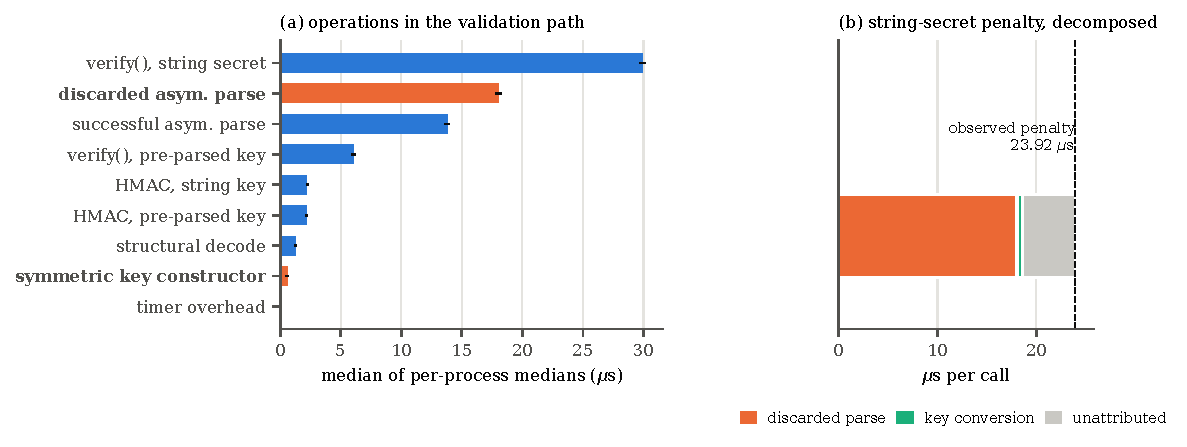
\includegraphics[width=\textwidth]{fig_decomposition.pdf}
\caption{(a) Every operation in Table~\ref{tab:host}, on a linear scale, with
the two components the paper turns on emphasised; whiskers are the 95\%
percentile bootstrap intervals over \HostInvocations{} processes. (b) The
\HostStringPenalty~$\mu$s penalty for supplying a string secret rather than a
pre-parsed key, decomposed. The three segments are medians of per-round paired
differences, not a partition of a single measurement, and they do not sum to the
penalty: the \DecompResidual~$\mu$s remainder is unattributed
(Section~\ref{sec:residual}).}
\label{fig:decomposition}
\end{figure*}

The two emphasised rows are the result. The signature primitive costs
\HostHmacString~$\mu$s of a \HostJwtString~$\mu$s call. The conversion to which
the remainder is most readily attributed costs
\HostCreateSecretKey~$\mu$s. The discarded attempt that precedes that conversion
costs \HostProbeThrows~$\mu$s, which is \HostProbeShareOfCall\% of the whole call
and its largest single component.

Supplying a pre-parsed key instead of a string reduces the call by
\HostStringPenalty~$\mu$s [\HostStringPenaltyCiLo, \HostStringPenaltyCiHi] over
\HostStringPenaltyRounds{} paired rounds.

\paragraph{Key conversion does not explain it} Once the signature primitive is
shown to be small, one explanation for the remainder suggests itself immediately:
that the cost lies in converting key material from a string into a key object on
every call. It is the natural explanation, and Table~\ref{tab:host} refutes
it. That conversion costs
\HostCreateSecretKey~$\mu$s, so the attribution is wrong by roughly the ratio
between that figure and \HostProbeThrows~$\mu$s.

A second observation is usually offered in support of the conversion account: an
asymmetry between HMAC and RSA costs, read as conversion being dearer than
parsing a PEM. It is backwards. A successful asymmetric parse costs
\HostProbeSucceeds~$\mu$s against \HostCreateSecretKey~$\mu$s for the
conversion. The real asymmetry is that the RSA path's parse \emph{succeeds},
making its cost useful work, while the HMAC path's fails, making it waste.

\subsection{What the \texorpdfstring{\HostProbeThrows~$\mu$s}{18 us} is made
of}\label{sec:granularity}

The \HostProbeThrows~$\mu$s is the cost of the discarded attempt taken whole. It
contains at least two things: the work OpenSSL performs before concluding that
the input is not an asymmetric key, and the construction and unwinding of the
exception that returns that conclusion to the library. Table~\ref{tab:host}
already bounds the split: a \emph{successful} asymmetric parse (the same
entry point, reaching a conclusion and throwing nothing) costs
\HostProbeSucceeds~$\mu$s, the same order as the failing one, so the exception
cannot be most of it. Table~\ref{tab:decomp} replaces the bound with a
decomposition, combining the C measurement of the same OpenSSL release
(Section~\ref{sec:c-method}) with the exception baseline
(Section~\ref{sec:exc-method}) on six official runtimes.

\begin{table*}[!t]
\caption{The discarded attempt decomposed, per runtime, in $\mu$s (x86\_64).
\emph{Probe}: \texttt{createPublicKey(secret)} inside Node, thrown and caught.
\emph{C parse}: the same OpenSSL calls issued from C against the OpenSSL
release that runtime bundles, built from source. \emph{V8 exception}: an
\texttt{Error} of the same shape, message and properties thrown from
\ExcDepth{} frames and discarded, with no OpenSSL call. \emph{Binding}: the
probe less the other two; its interval, from independent resampling of the
three runs, is in the replication package. Medians of per-process medians
over \ExcInvocations{} processes (probe, exception) and \CProbeInvocations{}
processes (C). The C column uses a stock build of each release, not Node's own
build of it, so the binding column is approximate (Section~\ref{sec:threats}).}
\label{tab:decomp}
\begin{tabular*}{\textwidth}{@{\extracolsep{\fill}}llrrrr@{}}
\toprule
Runtime & OpenSSL & Probe & C parse & V8 exception & Binding \\
\midrule
Node \RtEighteenLiteral & \RtEighteenOpenssl & \RtEighteenProbe & \RtEighteenDecompC & \RtEighteenExcNodeLike & \RtEighteenDecompLeftover \\
Node \RtTwentyLiteral & \RtTwentyOpenssl & \RtTwentyProbe & \RtTwentyDecompC & \RtTwentyExcNodeLike & \RtTwentyDecompLeftover \\
Node \RtTwentyThreeLiteral & \RtTwentyThreeOpenssl & \RtTwentyThreeProbe & \RtTwentyThreeDecompC & \RtTwentyThreeExcNodeLike & \RtTwentyThreeDecompLeftover \\
Node \RtTwentyTwoLiteral & \RtTwentyTwoOpenssl & \RtTwentyTwoProbe & \RtTwentyTwoDecompC & \RtTwentyTwoExcNodeLike & \RtTwentyTwoDecompLeftover \\
Node \RtTwentyFourLiteral & \RtTwentyFourOpenssl & \RtTwentyFourProbe & \RtTwentyFourDecompC & \RtTwentyFourExcNodeLike & \RtTwentyFourDecompLeftover \\
Node \RtTwentySixLiteral & \RtTwentySixOpenssl & \RtTwentySixProbe & \RtTwentySixDecompC & \RtTwentySixExcNodeLike & \RtTwentySixDecompLeftover \\
\bottomrule
\end{tabular*}
\end{table*}

Three things follow. First, on every runtime bundling OpenSSL~3.0 the C parse
alone matches the probe to within a few percent: \RtEighteenDecompCPct\% of
it under Node \RtEighteenLiteral{} and \RtTwentyThreeDecompCPct\% under Node
\RtTwentyThreeLiteral, the excess over 100\% being the difference between our
build of the release and Node's. There the discarded attempt \emph{is} the
OpenSSL parse, and it would cost the same with no JavaScript engine present.
Second, the exception is small and nearly constant across runtimes: the
Node-shaped error costs \RtEighteenExcNodeLike~$\mu$s under Node
\RtEighteenLiteral{} and \RtTwentySixExcNodeLike~$\mu$s under Node
\RtTwentySixLiteral{} (\RtEighteenDecompExcPct\% and
\RtTwentySixDecompExcPct\% of the respective probes), and roughly half of it
is stack capture (with capture disabled, \RtEighteenExcNoStack{} and
\RtTwentySixExcNoStack~$\mu$s). Disabling stack capture for the real probe
saves \RtEighteenStackCapture~$\mu$s and \RtTwentySixStackCapture~$\mu$s on
the same two runtimes, the same order as the synthetic figure. Third, on
runtimes bundling OpenSSL~3.5, where the parse is cheap, the three parts are of
comparable size: under Node \RtTwentySixLiteral{} the parse is
\RtTwentySixDecompCPct\% of the probe, the exception \RtTwentySixDecompExcPct\%
and the binding \RtTwentySixDecompLeftoverPct\%.

The component is therefore a discarded \emph{parse attempt}, not an exception
cost. Where it is expensive the exception is about a
hundredth of it, and even where it is cheap the exception is a fifth. These
runtimes are Linux builds on x86\_64; the ARM64 host figure of
Table~\ref{tab:host} was not itself decomposed this way, and its
\HostProbeThrows~$\mu$s is of the same order as the OpenSSL~3.5 rows here, not
the OpenSSL~3.0 rows.

\subsection{Checks on the decomposition}\label{sec:residual}

The discarded parse and the conversion together account for
\DecompExplainedPct\% of the \DecompObserved~$\mu$s string penalty; the
\DecompResidual~$\mu$s residual [\DecompResidualCiLo, \DecompResidualCiHi] lies
in the library's own type and claim checking and is reported as unattributed
rather than absorbed into the headline. Because the decomposition relies on
differencing, it was also checked against V8's sampling profiler, which needs
no arithmetic on our part: the asymmetric key parse accounts for a median
\ProfHostPct\% of self time on the host, \ProfEighteenPct\% under Node
\NodeEighteenNodeMajor{} and \ProfTwentySixPct\% under Node
\NodeTwentySixMuslNodeMajor, and does not appear among the top frames of the
pre-parsed path. Two methods, one answer (Supplementary Section~S3).

%% ============================================================================
\section{RQ2: What governs the magnitude}\label{sec:rq2}

Table~\ref{tab:matrix} varies the runtime with containerisation held constant,
and Figure~\ref{fig:matrix} plots the two columns that matter.

\begin{table*}[!htbp]
\caption{The same measurement across four container runtimes on one machine,
\MatrixInvocations{} processes each of \MatrixCallsPerInvocation{} calls. The
\emph{Disc.\ parse}: the discarded asymmetric parse; \emph{Pre-parsed}:
\texttt{verify()} with a pre-parsed key. $^{\ddagger}$The host row is from
Table~\ref{tab:host} and is not containerised.
$^{\dagger}$Inferred from the run timestamp, not recorded per row: that run
predates the per-measurement OpenSSL field (Section~\ref{sec:threats}).}
\label{tab:matrix}
\begin{tabular*}{\textwidth}{@{\extracolsep{\fill}}lllrr@{}}
\toprule
Runtime & OpenSSL & V8 & Disc.\ parse & Pre-parsed \\
        &         &    & ($\mu$s)     & ($\mu$s) \\
\midrule
Node \NodeEighteenNodeMajor{} musl        & \NodeEighteenOpensslLiteral       & \NodeEighteenVeight       & \NodeEighteenProbeThrows       & \NodeEighteenJwtPreparsed \\
Node \NodeTwentyNodeMajor{} musl          & \NodeTwentyOpensslLiteral         & \NodeTwentyVeight         & \NodeTwentyProbeThrows         & \NodeTwentyJwtPreparsed \\
Node \NodeTwentySixMuslNodeMajor{} musl   & \NodeTwentySixMuslOpensslLiteral  & \NodeTwentySixMuslVeight  & \NodeTwentySixMuslProbeThrows  & \NodeTwentySixMuslJwtPreparsed \\
Node \NodeTwentySixGlibcNodeMajor{} glibc & \NodeTwentySixGlibcOpensslLiteral & \NodeTwentySixGlibcVeight & \NodeTwentySixGlibcProbeThrows & \NodeTwentySixGlibcJwtPreparsed \\
host$^{\ddagger}$                         & \HostOpensslInferred$^{\dagger}$  & \HostVeight               & \HostProbeThrows               & \HostJwtPreparsed \\
\bottomrule
\end{tabular*}
\end{table*}

\begin{figure*}[!t]
\centering
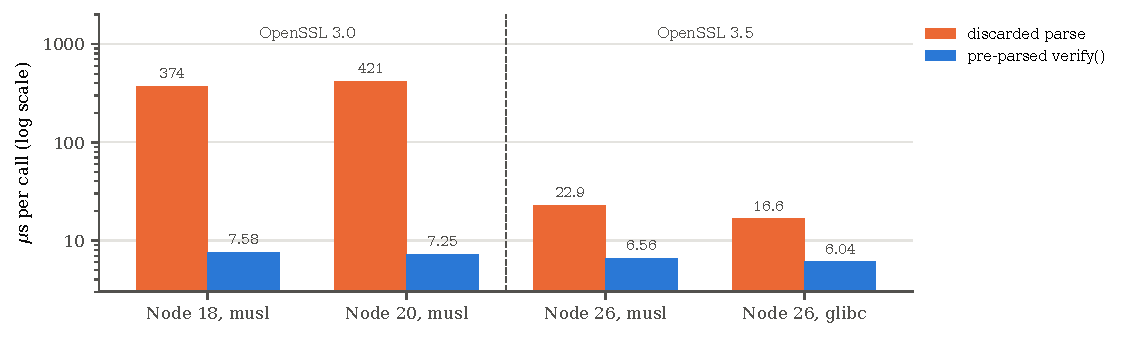
\includegraphics[width=\textwidth]{fig_runtime_matrix.pdf}
\caption{The four container rows of Table~\ref{tab:matrix} on a logarithmic
axis. The discarded parse spans \SpanProbeThrows$\times$ across images while the
pre-parsed call spans \SpanJwtPreparsed$\times$. The dashed rule marks the
OpenSSL series boundary. Within this matrix it is not a controlled boundary,
because the two fast images also carry a newer engine and a different build
(Section~\ref{sec:cannot-separate}); Section~\ref{sec:rq2-causal} controls it. The uncontainerised host row is omitted
because its comparison with the container rows is confounded.}
\label{fig:matrix}
\end{figure*}

\subsection{What the matrix shows, and what it cannot separate}\label{sec:cannot-separate}

Node \NodeEighteenNodeMajor{} and Node \NodeTwentyNodeMajor{} ship different
major versions of V8 (\NodeEighteenVeight{} and \NodeTwentyVeight) and share the
OpenSSL \NodeEighteenOpensslSeries{} series; both pay of order
\NodeEighteenProbeThrows--\NodeTwentyProbeThrows~$\mu$s, so within that series
the engine does not move the quantity. The effect is confined to key parsing:
across the four container rows pre-parsed validation spans
\SpanJwtPreparsed$\times$ and the HMAC primitive \SpanHmacString$\times$, while
the discarded parse spans \SpanProbeThrows$\times$ and a successful parse moves
with it (\SpanProbeSucceeds$\times$). The matrix cannot, however, separate
OpenSSL from the engine across the series boundary, because the fast images
also carry a newer engine and a different build; nor does it isolate
containerisation (Supplementary Section~S4). The causal wording in this paper
rests on the crossed designs below, not on the matrix.

\subsection{Caused by OpenSSL: the parse without an engine}\label{sec:rq2-causal}

Table~\ref{tab:cprobe} removes Node entirely: the OpenSSL calls
\texttt{createPublicKey()} makes for an HMAC secret, issued from C against
\CProbeVersionCount{} OpenSSL releases built identically, and
Figure~\ref{fig:openssl} plots its first and last columns.

\begin{figure}[!t]
\centering
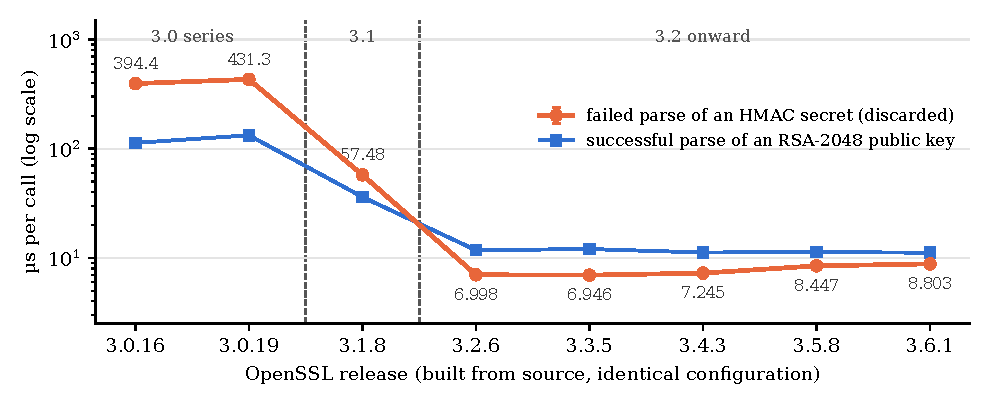
\includegraphics[width=\linewidth]{fig_openssl_releases.pdf}
\caption{The failed parse of an HMAC secret issued from C, with no JavaScript
engine, against \CProbeVersionCount{} OpenSSL releases built from source with
one configuration (Table~\ref{tab:cprobe}, column \emph{Full}), beside a
successful parse of an RSA-2048 public key through the same path. Whiskers are
95\% percentile bootstrap intervals over \CProbeInvocations{} processes and
are narrower than the markers. The cost falls in two steps, at 3.1 and 3.2,
and is flat thereafter.}
\label{fig:openssl}
\end{figure}

\begin{table*}[!t]
\caption{The failed asymmetric parse issued from C, with no JavaScript engine,
against \CProbeVersionCount{} OpenSSL releases built from source with one
compiler and one set of flags (x86\_64), in $\mu$s. Medians of per-process
medians over \CProbeInvocations{} processes of \CProbeCallsPerInvocation{}
calls. \emph{Full}: everything \texttt{createPublicKey()} asks of OpenSSL for
an HMAC secret, including the error-string drain; 95\% intervals for it are in
the replication package and are within \CFullCiMaxHalfWidthPct\% of the median for every release.
Its parts follow. \emph{Successful parse}: an RSA-2048 public key through the
same path, for comparison.}
\label{tab:cprobe}
\begin{tabular*}{\textwidth}{@{\extracolsep{\fill}}lrrrrr@{}}
\toprule
        &      & Private-key & Public-key & Error   & Successful \\
OpenSSL & Full & parse       & scans      & strings & parse \\
\midrule
\CVersionLiteralVThreeZeroSixteen & \CFullVThreeZeroSixteen & \CPrivateParseVThreeZeroSixteen & \CPublicTriesVThreeZeroSixteen & \CErrorStringsVThreeZeroSixteen & \CSpkiOkVThreeZeroSixteen \\
\CVersionLiteralVThreeZeroNineteen & \CFullVThreeZeroNineteen & \CPrivateParseVThreeZeroNineteen & \CPublicTriesVThreeZeroNineteen & \CErrorStringsVThreeZeroNineteen & \CSpkiOkVThreeZeroNineteen \\
\CVersionLiteralVThreeOneEight & \CFullVThreeOneEight & \CPrivateParseVThreeOneEight & \CPublicTriesVThreeOneEight & \CErrorStringsVThreeOneEight & \CSpkiOkVThreeOneEight \\
\CVersionLiteralVThreeTwoSix & \CFullVThreeTwoSix & \CPrivateParseVThreeTwoSix & \CPublicTriesVThreeTwoSix & \CErrorStringsVThreeTwoSix & \CSpkiOkVThreeTwoSix \\
\CVersionLiteralVThreeThreeFive & \CFullVThreeThreeFive & \CPrivateParseVThreeThreeFive & \CPublicTriesVThreeThreeFive & \CErrorStringsVThreeThreeFive & \CSpkiOkVThreeThreeFive \\
\CVersionLiteralVThreeFourThree & \CFullVThreeFourThree & \CPrivateParseVThreeFourThree & \CPublicTriesVThreeFourThree & \CErrorStringsVThreeFourThree & \CSpkiOkVThreeFourThree \\
\CVersionLiteralVThreeFiveEight & \CFullVThreeFiveEight & \CPrivateParseVThreeFiveEight & \CPublicTriesVThreeFiveEight & \CErrorStringsVThreeFiveEight & \CSpkiOkVThreeFiveEight \\
\CVersionLiteralVThreeSixOne & \CFullVThreeSixOne & \CPrivateParseVThreeSixOne & \CPublicTriesVThreeSixOne & \CErrorStringsVThreeSixOne & \CSpkiOkVThreeSixOne \\
\bottomrule
\end{tabular*}
\end{table*}

In plain C the failure costs \CFullVThreeZeroSixteen~$\mu$s on OpenSSL \CVersionLiteralVThreeZeroSixteen{}
and \CFullVThreeFiveEight~$\mu$s on \CVersionLiteralVThreeFiveEight, a ratio of \CFullRatioOldNew{}
[\CFullRatioOldNewCiLo, \CFullRatioOldNewCiHi]. Nothing else differs between
those two measurements: the program, the compiler, the flags, the machine and
the protocol are the same. The magnitude is therefore \emph{caused} by the
OpenSSL release. That is a claim about this code path in these releases; it
says nothing about OpenSSL performance generally.

The table also says where in OpenSSL the cost lives and when it went away.
Almost all of it is the private-key parse (\CPrivateShareVThreeZeroSixteen\%
of the full sequence on \CVersionLiteralVThreeZeroSixteen{}), the step at which OpenSSL~3 hands the input
to its provider-based decoders; the three public-key scans reject the input at
the PEM header and are cheap in every release, and the error strings cost under
a microsecond. The fall came in two steps: to \CFullVThreeOneEight~$\mu$s in
\CVersionLiteralVThreeOneEight, and to \CFullVThreeTwoSix~$\mu$s in \CVersionLiteralVThreeTwoSix, after which it is flat to
within a few microseconds through \CProbeVersionLast. We measured the steps,
not the source changes that produced them; identifying those would take a
bisection of the OpenSSL history that we have not done. A successful parse of
real key material fell with it, which is why the effect is confined to key
parsing in general rather than to the failure path.

\paragraph{Engine and library crossed} The official runtimes of
Section~\ref{sec:exc-method} contain the pairing stock container images lack:
Node \RtTwentyTwoLiteral{} ships V8 \RtTwentyTwoVeightFull{} with OpenSSL
\RtTwentyTwoOpenssl, while Node \RtTwentyThreeLiteral{} ships the \emph{newer}
V8 \RtTwentyThreeVeightFull{} with the \emph{older} OpenSSL
\RtTwentyThreeOpenssl. The probe costs \RtTwentyTwoProbe~$\mu$s on the first
and \RtTwentyThreeProbe~$\mu$s on the second. The Node \NodeEighteenNodeMajor/\NodeTwentyNodeMajor{} pair of
Table~\ref{tab:matrix} showed that a change of engine at a fixed OpenSSL series
leaves the cost where it was; this pair shows that a newer engine does not
rescue an older OpenSSL. Together with the C measurement, the engine is
excluded from both directions.

\subsection{A second architecture}\label{sec:rq2-arch}

The runtime matrix and the host decomposition were repeated with the same
images and scripts on x86\_64 (Section~\ref{sec:arch-method}). The property the
attribution rests on, every OpenSSL~3.0 image slower than every OpenSSL~3.5
image, \XmSeriesSplitHolds{} there too: the discarded parse spans
\XmSpanProbeThrows$\times$ across the images while pre-parsed validation spans
\XmSpanJwtPreparsed$\times$. The host decomposition keeps its ordering: the
discarded parse is \XhProbeThrows~$\mu$s of a \XhJwtString~$\mu$s call
(\XhProbeShareOfCall\%). The full table is in Supplementary Section~S4.

%% ============================================================================
\section{RQ3: The containerised service, and prevalence}\label{sec:rq3}

\subsection{In-situ cost across arrival rates}\label{sec:insitu}

The containerised service was driven at seven arrival rates, each measured by the
paired-scrape difference of Section~\ref{sec:insitu-method}, with the whole sweep
run ascending and then descending on one process. Figure~\ref{fig:insitu}
plots both passes at each rate for the configuration the service deploys, a
string secret (the values are tabulated in Supplementary Section~S5).

\begin{figure}[!t]
\centering
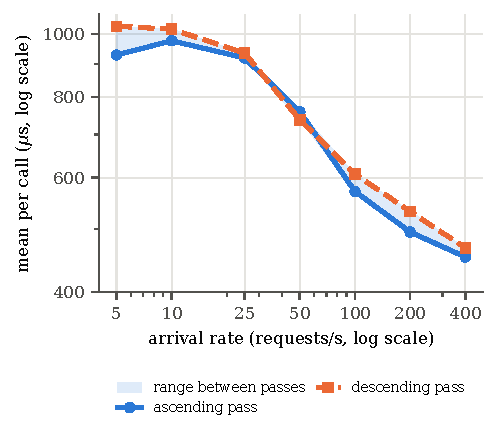
\includegraphics[width=0.72\columnwidth]{fig_insitu_rate.pdf}
\caption{In-situ validation cost against arrival rate, string secret. The two
passes are drawn separately rather than averaged: Supplementary Section~S5 reports
that they differ systematically, and averaging would conceal that. The shaded
band is the range between the passes, which is two observations rather than an
interval.}
\label{fig:insitu}
\end{figure}

One observation follows, and it is the one this section claims: the cost is
present in the containerised service and is far larger than the isolated host figure of
Table~\ref{tab:host}, consistent with Section~\ref{sec:rq2} in that the service's
runtime is the one carrying the older OpenSSL.

Two things in these measurements need care, and we set them out
explicitly.

\paragraph{Wall-clock exceeds the prediction; processor time does not} The
service runtime's discarded parse costs \NodeEighteenProbeThrows~$\mu$s
(Table~\ref{tab:matrix}), and the remainder of the validation path is of order
\NodeEighteenJwtPreparsed~$\mu$s, giving an expected total near
\InsituPredictedFromMatrix~$\mu$s. The wall-clock means observed across the
sweep are \InsituObservedLo--\InsituObservedHi~$\mu$s, exceeding that by
\InsituUnaccountedLo--\InsituUnaccountedHi~$\mu$s. Contention inflates a
duration rather than deflating it, so these are upper bounds, and
Section~\ref{sec:abcorroboration} shows where the excess is not: measured as
processor time, the validation call costs within \AbCpuVsPredictedPct\% of the
prediction. The excess is therefore time the call spent off the processor on a
shared host, not additional work. We did not decompose that off-processor time
further, and no claim below depends on it.

\paragraph{Neither the decline with rate nor the gap between passes is
interpreted} Cost falls from \InsituStringAscA~$\mu$s at
\InsituRateA~requests/s to \InsituStringAscG~$\mu$s at
\InsituRateG~requests/s, and the two passes differ systematically rather than
randomly. Several mechanisms unrelated to validation could produce either, we
did not run the conditions that would distinguish them, and no claim here
depends on them (Supplementary Section~S5).

\subsection{Corroboration: the cost is processor time, and it matches the
prediction}\label{sec:abcorroboration}

An in-situ figure of this magnitude has two readings. Either it is work the
service performs, or it is time the request spends waiting, queued behind
other requests, descheduled by a contended host, or inflated by the instrument.
We separate them with an A/B of the same service at one arrival rate, with
validation enabled in one window and disabled in the next, on the same pod
running the same image, and read the processor time the application container
was charged from its cgroup accounting rather than from a clock.
Table~\ref{tab:ab} reports it.

\begin{table*}[!htbp]
\caption{Validation enabled against validation disabled, at one arrival rate,
two \AbWindowSecondsJwt~s windows on the same pod and image, \AbRequestsNone{}
requests each. A signed token is on the wire in both arms; the disabled arm
removes only the handler's \texttt{jwt.verify()} call. Application and sidecar
CPU are means of one-second cgroup samples in the window; CPU per call is that
mean divided by the achieved rate. Event-loop lag is the mean of the
per-scrape p99. Host load is a single sample at window start.}
\label{tab:ab}
\begin{tabular*}{\textwidth}{@{\extracolsep{\fill}}lrr@{}}
\toprule
 & disabled & enabled \\
\midrule
Achieved rate (req/s)              & \AbRateNone                & \AbRateJwt \\
Application CPU (millicores)       & \AbCpuNone                 & \AbCpuJwt \\
\textbf{CPU per call ($\mu$s)}     & \textbf{\AbCpuPerCallNone} & \textbf{\AbCpuPerCallJwt} \\
Sidecar CPU (millicores)           & \AbSidecarCpuNone          & \AbSidecarCpuJwt \\
Event-loop lag (ms)                & \AbEventLoopLagNone        & \AbEventLoopLagJwt \\
Client mean latency (ms)           & \AbLatencyNone             & \AbLatencyJwt \\
Host load, 1 min                   & \AbLoadOneNone             & \AbLoadOneJwt \\
\bottomrule
\end{tabular*}
\end{table*}

Enabling validation adds \AbCpuPerCallDelta~$\mu$s of processor time per
call. The runtime matrix predicts \InsituPredictedFromMatrix~$\mu$s for the same
work on the same runtime (Section~\ref{sec:insitu}); the two agree to within
\AbCpuVsPredictedPct\%. They are obtained by instruments that share no code:
cgroup CPU accounting on the service's pod, and a single-process microbenchmark
in an isolated container. A request that queues or is descheduled accrues
wall-clock time but no CPU, so this figure cannot contain queueing delay.

Three observations weigh against reading the difference as an artefact of the
two windows. The sidecar, in the same pod under the same contention, did not
rise with the application: \AbSidecarCpuNone{} millicores disabled against
\AbSidecarCpuJwt{} enabled. The one-second CPU samples of the two arms do not
overlap at all (disabled never exceeded \AbCpuSampleMaxNone{} millicores in
\AbCpuSamplesNone{} samples, enabled never fell below \AbCpuSampleMinJwt{} in
\AbCpuSamplesJwt{}), which separates the arms without a distributional
assumption. And event-loop lag is unchanged, so neither arm was near
saturation. The two windows are two observations, not a sample: the difference
carries no interval and we compute none.


\subsection{How common is the avoiding pattern, in our
sample?}\label{sec:prevalence}

Three instruments, three frames, reported separately as Section~\ref{sec:frames}
requires. All counts were captured on \PopCapturedAt. None of the figures below
is a population proportion.

\paragraph{Population co-occurrence} In code-search counts over public
repositories, no cell exceeds \PopWorstCellPct\% of files importing the library
that also mention the pre-parsing interface (Supplementary Section~S5).

\begin{figure}[!t]
\centering
%% Where the secret passed to verify() comes from, in the classified sample.
%% Every count is a macro from keypath_macros.tex.
\begingroup
\definecolor{svbar}{HTML}{2F6FD0}
\definecolor{svzero}{HTML}{E8663A}
\begin{tikzpicture}
\begin{axis}[
  xbar, bar width=8pt, bar shift=0pt,
  width=0.8\linewidth, height=58mm,
  xmin=0, xmax=210,
  xlabel={Call sites (of \SampleCallSites{}, in \SampleRepos{} repositories)},
  xlabel style={font=\footnotesize},
  symbolic y coords={env,unknown,literal,file,buffer,preparsed},
  ytick={env,unknown,literal,file,buffer,preparsed}, y dir=reverse,
  yticklabels={Environment variable (string), Untraced identifier,
    String literal, File contents, Buffer, \textbf{Pre-parsed key object}},
  yticklabel style={font=\scriptsize},
  xticklabel style={font=\scriptsize},
  enlarge y limits=0.12,
  nodes near coords, nodes near coords align={horizontal},
  every node near coord/.append style={font=\scriptsize, text=black},
  axis x line*=bottom, axis y line*=left,
  xmajorgrids, grid style={draw=black!10},
]
\addplot[fill=svbar, draw=svbar] coordinates {
  (\SampleEnvString,env) (\SampleUnknown,unknown) (\SampleStringLiteral,literal)
  (\SampleFileContents,file) (\SampleBuffer,buffer)};
\addplot[fill=svzero, draw=svzero, forget plot] coordinates {
  (\SampleSitesPreparsed,preparsed)};
\end{axis}
\end{tikzpicture}
\endgroup

\caption{Where the secret passed to the validator comes from, for the
\SampleCallSites{} call sites classified in our sample. No call site passes a
pre-parsed key object, the one form that avoids the discarded parse for every
input. Independently, \SampleNoAlgorithms{} of the \SampleCallSites{} call
sites (\SampleNoAlgorithmsPct\%) pass no algorithm restriction. Counts
describe the sample, not the population (Section~\ref{sec:frames}).}
\label{fig:survey}
\end{figure}

\paragraph{Classified call sites} Of \SampleCallSites{} call sites classified
across \SampleRepos{} distinct repositories in our sample,
\SampleSitesPreparsed{} pass a pre-parsed key. Environment variables account for
\SampleEnvString{} of those call sites, untraced identifiers and member
expressions \SampleUnknown{}, string literals \SampleStringLiteral{}, file
contents \SampleFileContents{} and buffers \SampleBuffer{}
(Figure~\ref{fig:survey}). No file in this corpus
contains the pre-parsing interface at all, in any spelling, so the zero reflects
the pattern's absence from the sample rather than a classifier that cannot see
it. Incidentally, \SampleNoAlgorithms{} of \SampleCallSites{} call sites
(\SampleNoAlgorithmsPct\%) pass no algorithm restriction, which
Section~\ref{sec:fix} returns to.

\paragraph{Targeted counter-search} A sample can only show a pattern is rare if
it could have found it. Every file co-occurring the library with the pre-parsing
interface was therefore fetched: \CounterFilesFetched{} files, of which
\CounterWithVerify{} contain a validation call, spanning
\CounterReposWithVerify{} distinct repositories. An automated pass flagged
\AdjudicatedTotal{} call sites as passing a pre-parsed key and all were then read
by hand: \AdjudicatedFalsePositive{} are false positives (projects defining
their own helper function of the same name, one of which returns a string),
\AdjudicatedUnresolved{} could not be resolved within its file, and
\AdjudicatedGenuine{} are genuine, across \AdjudicatedGenuineProjects{} distinct
projects.

\paragraph{The rate, with its denominator} Among the \CounterReposWithVerify{}
repositories that both reference the pre-parsing interface and call the
validator, \AdjudicatedGenuineProjects{} use it: \AdjudicatedGenuinePct\%. That
denominator is the most favourable available, since those projects demonstrably
know the interface exists, and it is not the population. Within this frame the
pattern is rare rather than absent, and it is rare even among projects already
aware of it. We do not extrapolate beyond the frame.

%% ============================================================================
\section{RQ4: One library, or a design choice?}\label{sec:rq4}

A cost found in one library is an observation about that library. It becomes a
statement about a class of defect only if the mechanism can be named
independently of the library and predicts which other libraries have it. The
mechanism here can be named: \emph{resolving key material of unknown type by
attempting the asymmetric parse first, and treating its failure as the signal
that the material is a shared secret}. Table~\ref{tab:xlib} tests the
prediction against six further libraries.

\begin{table*}[!t]
\caption{HS256 verification across seven JWT libraries in four languages
(x86\_64), in $\mu$s. \emph{Asym.\ first?}: given a string HMAC secret, does
the library attempt to parse it as an asymmetric key, as read from its source.
\emph{String} and \emph{pre-parsed}: the secret in the form the library's
documentation shows, and in the library's own key object built once
(Section~\ref{sec:xlib-method}). \emph{Penalty}: median of per-round paired
differences, with a 95\% bootstrap interval over rounds. Medians of
per-process medians over \XlibInvocations{} processes of
\XlibCallsPerInvocation{} calls. Absolute costs measure different amounts of
work in different runtimes and are not a ranking of libraries.
$^{a}$No string accepted for an HMAC key; the rawest accepted form (bytes) is
used. $^{b}$A string is accepted only by a deprecated setter that resolves it
once, when the parser is built.}
\label{tab:xlib}
\footnotesize\setlength{\tabcolsep}{3pt}
\resizebox{\textwidth}{!}{%
\begin{tabular}{@{}lllllrrrl@{}}
\toprule
Library & Lang. & Version & Crypto backend & Asym.\ first? & String & Pre-parsed & Penalty & 95\% interval \\
\midrule
\texttt{jsonwebtoken} & JS & \XlibJsonwebtokenOldSslVersion & \XlibJsonwebtokenOldSslBackend & \textbf{yes} & \XlibJsonwebtokenOldSslString & \XlibJsonwebtokenOldSslPreparsed & \XlibJsonwebtokenOldSslPenalty & [\XlibJsonwebtokenOldSslPenaltyCiLo, \XlibJsonwebtokenOldSslPenaltyCiHi] \\
\texttt{jsonwebtoken} & JS & \XlibJsonwebtokenNewSslVersion & \XlibJsonwebtokenNewSslBackend & \textbf{yes} & \XlibJsonwebtokenNewSslString & \XlibJsonwebtokenNewSslPreparsed & \XlibJsonwebtokenNewSslPenalty & [\XlibJsonwebtokenNewSslPenaltyCiLo, \XlibJsonwebtokenNewSslPenaltyCiHi] \\
\texttt{fast-jwt} & JS & \XlibFastjwtOldSslVersion & \XlibFastjwtOldSslBackend & no & \XlibFastjwtOldSslString & \XlibFastjwtOldSslPreparsed & \XlibFastjwtOldSslPenalty & [\XlibFastjwtOldSslPenaltyCiLo, \XlibFastjwtOldSslPenaltyCiHi] \\
\texttt{fast-jwt} & JS & \XlibFastjwtNewSslVersion & \XlibFastjwtNewSslBackend & no & \XlibFastjwtNewSslString & \XlibFastjwtNewSslPreparsed & \XlibFastjwtNewSslPenalty & [\XlibFastjwtNewSslPenaltyCiLo, \XlibFastjwtNewSslPenaltyCiHi] \\
\texttt{jose} & JS & \XlibJoseOldSslVersion & \XlibJoseOldSslBackend & no$^{a}$ & \XlibJoseOldSslString & \XlibJoseOldSslPreparsed & \XlibJoseOldSslPenalty & [\XlibJoseOldSslPenaltyCiLo, \XlibJoseOldSslPenaltyCiHi] \\
\texttt{jose} & JS & \XlibJoseNewSslVersion & \XlibJoseNewSslBackend & no$^{a}$ & \XlibJoseNewSslString & \XlibJoseNewSslPreparsed & \XlibJoseNewSslPenalty & [\XlibJoseNewSslPenaltyCiLo, \XlibJoseNewSslPenaltyCiHi] \\
\texttt{PyJWT} & Python & \XlibPyjwtVersion & \XlibPyjwtBackend & no & \XlibPyjwtString & \XlibPyjwtPreparsed & \XlibPyjwtPenalty & [\XlibPyjwtPenaltyCiLo, \XlibPyjwtPenaltyCiHi] \\
\texttt{golang-jwt} & Go & \XlibGolangjwtVersion & \XlibGolangjwtBackend & no$^{a}$ & \XlibGolangjwtString & \XlibGolangjwtPreparsed & \XlibGolangjwtPenalty & [\XlibGolangjwtPenaltyCiLo, \XlibGolangjwtPenaltyCiHi] \\
\texttt{nimbus-jose-jwt} & Java & \XlibNimbusVersion & \XlibNimbusBackend & no & \XlibNimbusString & \XlibNimbusPreparsed & \XlibNimbusPenalty & [\XlibNimbusPenaltyCiLo, \XlibNimbusPenaltyCiHi] \\
\texttt{jjwt} & Java & \XlibJjwtVersion & \XlibJjwtBackend & no$^{b}$ & \XlibJjwtString & \XlibJjwtPreparsed & \XlibJjwtPenalty & [\XlibJjwtPenaltyCiLo, \XlibJjwtPenaltyCiHi] \\
\bottomrule
\end{tabular}}
\end{table*}

\begin{figure}[!t]
\centering
%% String-to-pre-parsed cost ratio across seven JWT libraries (Table xlib).
%% Every coordinate is a macro from revision_macros.tex; no value is typed here.
\begingroup
\definecolor{xlpay}{HTML}{E8663A}
\definecolor{xlfree}{HTML}{8A8984}
\begin{tikzpicture}
\begin{axis}[
  xbar, xmode=log, log basis x=10,
  width=0.78\linewidth, height=80mm,
  legend style={font=\scriptsize, at={(0.5,-0.2)}, anchor=north, legend columns=2, draw=none},
  bar width=6pt, bar shift=0pt, enlarge y limits=0.07,
  xmin=0.5, xmax=150, log origin=infty,
  xlabel={Cost with a raw secret $\div$ cost with a pre-parsed key (log scale)},
  symbolic y coords={jwtO,jwtN,joseO,joseN,fastjwtO,fastjwtN,pyjwt,golangjwt,nimbus,jjwt},
  ytick={jwtO,jwtN,joseO,joseN,fastjwtO,fastjwtN,pyjwt,golangjwt,nimbus,jjwt}, y dir=reverse,
  yticklabels={
    {\texttt{jsonwebtoken}, OpenSSL~3.0},
    {\texttt{jsonwebtoken}, OpenSSL~3.5},
    {\texttt{jose}, OpenSSL~3.0},
    {\texttt{jose}, OpenSSL~3.5},
    {\texttt{fast-jwt}, OpenSSL~3.0},
    {\texttt{fast-jwt}, OpenSSL~3.5},
    {\texttt{PyJWT}},
    {\texttt{golang-jwt}},
    {\texttt{nimbus-jose-jwt}},
    {\texttt{jjwt}}},
  yticklabel style={font=\scriptsize, align=right},
  xticklabel style={font=\scriptsize},
  xlabel style={font=\footnotesize},
  xtick={0.5,1,2,5,10,20,50,100},
  xticklabels={0.5,1,2,5,10,20,50,100},
  nodes near coords, nodes near coords align={horizontal},
  every node near coord/.append style={font=\scriptsize, text=black},
  point meta=explicit symbolic,
  axis x line*=bottom, axis y line*=left,
  xmajorgrids, grid style={draw=black!10},
  extra x ticks={1}, extra x tick labels={},
  extra x tick style={grid style={draw=black!50, dashed}},
]
\addplot[fill=xlpay, draw=xlpay] coordinates {
  (\XlibJsonwebtokenOldSslRatio,jwtO) [\XlibJsonwebtokenOldSslRatio$\times$]
  (\XlibJsonwebtokenNewSslRatio,jwtN) [\XlibJsonwebtokenNewSslRatio$\times$]
  (\XlibJoseOldSslRatio,joseO)        [\XlibJoseOldSslRatio$\times$]
  (\XlibJoseNewSslRatio,joseN)        [\XlibJoseNewSslRatio$\times$]
};
\addplot[fill=xlfree, draw=xlfree] coordinates {
  (\XlibFastjwtOldSslRatio,fastjwtO) [\XlibFastjwtOldSslRatio$\times$]
  (\XlibFastjwtNewSslRatio,fastjwtN) [\XlibFastjwtNewSslRatio$\times$]
  (\XlibPyjwtRatio,pyjwt)            [\XlibPyjwtRatio$\times$]
  (\XlibGolangjwtRatio,golangjwt)    [\XlibGolangjwtRatio$\times$]
  (\XlibNimbusRatio,nimbus)          [\XlibNimbusRatio$\times$]
  (\XlibJjwtRatio,jjwt)              [\XlibJjwtRatio$\times$]
};
\legend{{Paired penalty interval excludes zero},{Interval includes zero}}
\end{axis}
\end{tikzpicture}
\endgroup

\caption{How much each library pays for being handed its raw secret rather
than its own pre-parsed key object: the ratio of the two costs in
Table~\ref{tab:xlib}, on a log scale. A ratio of one (dashed line) means no
per-call penalty. Orange: the paired 95\% interval on the penalty excludes
zero. Only \LibraryName{} performs the failing asymmetric parse, and only it
pays by more than a small factor; \texttt{jose} pays for re-importing raw bytes
on every call.}
\label{fig:xlib}
\end{figure}

\paragraph{What the source says} Only \LibraryName{} attempts the asymmetric
parse. The others resolve the ambiguity in one of three ways, none of which
involves a parse that can fail on a shared secret.
\emph{Inspect, then dispatch:} \texttt{fast-jwt} examines the text of the key
(whether it carries a PEM header or is a JSON Web Key) and calls exactly
one constructor, skipping even that inspection when every permitted algorithm
is HMAC; \texttt{PyJWT} likewise inspects the text, and rejects PEM- or
SSH-looking material offered as an HMAC key rather than trying to parse it.
\emph{Refuse the ambiguous input:} \texttt{jose} does not accept a string for an
HMAC key, and \texttt{golang-jwt} accepts only a byte slice for HMAC
verification, returning a key-type error for anything else.
\emph{Type the key:} \texttt{jjwt} requires a \texttt{SecretKey} for HMAC and a
\texttt{PublicKey} for signatures, so the distinction is made by the Java type
system; \texttt{nimbus-jose-jwt} offers a constructor that takes a string and
converts its bytes without parsing them. Refusing a string does not by itself
remove per-call work, however: \texttt{jose}, handed raw bytes, imports them
into a WebCrypto key on every call.

\paragraph{What the measurements say} Of the \XlibLibCount{} libraries,
\XlibPenaltyLibCount{} pay for being handed their raw form rather than a key
object, in the sense that the paired interval on the penalty excludes zero; for
the other \XlibZeroPenaltyLibCount{} it does not, and their point estimates are
within a microsecond of zero. The two are \LibraryName{} and \texttt{jose}, and
they pay for different reasons. \LibraryName{} performs the failing asymmetric
parse: its penalty is \XlibJsonwebtokenOldSslPenalty~$\mu$s under
\XlibJsonwebtokenOldSslBackend{} and \XlibJsonwebtokenNewSslPenalty~$\mu$s under
\XlibJsonwebtokenNewSslBackend, a string-to-pre-parsed ratio of
\XlibJsonwebtokenOldSslRatio{} and \XlibJsonwebtokenNewSslRatio{}
respectively (Figure~\ref{fig:xlib}). \texttt{jose} parses nothing that can fail, but imports the raw
bytes into a WebCrypto key on every call: \XlibJoseOldSslPenalty~$\mu$s and
\XlibJoseNewSslPenalty~$\mu$s under the same two runtimes. Both penalties grow
on OpenSSL~3.0, so the OpenSSL release sets the price of per-call key handling
generally; but the failing parse is the costliest form of it, about
\XlibJwtOverJoseOldSsl{} times \texttt{jose}'s on OpenSSL~3.0. Two of the
libraries that pay nothing resolve the key once, when a verifier or parser is
built (\texttt{fast-jwt}, \texttt{jjwt}), so a raw secret costs nothing per
call by construction; that is itself the design point.

\paragraph{What this establishes} The libraries without the problem matter as
much as the ones with it. All seven validate the same kind of token with the
same primitive (against the same OpenSSL, in the JavaScript cases) and
five pay nothing for a raw secret. The cost therefore follows a design choice,
resolving key material on every call, and not JSON Web Token validation, HMAC
or OpenSSL as such: OpenSSL~3.0 sets the price, but only a library that makes
that choice is charged it, and one that makes it by way of a failing parse is
charged the most. The failing parse is exactly what the order-of-evaluations
profiler of \citet{selakovic2017actionable} is designed to
find, and the alternatives above are the fixes that line of work suggests:
reorder the test, make it cheap, or move it off the per-call path. The
comparison does not estimate how many libraries make the choice; it shows that
making it is what matters.

%% ============================================================================
\section{RQ5: Removing the cost safely}\label{sec:security}

Sections~\ref{sec:rq1}--\ref{sec:rq4} treat the discarded attempt as a cost.
This section asks who can cause it, why it is there, and what removing it does
to the library's defences. Its evidence is the library's source at the
releases named, the library's own test suite, and the measurements already
reported; it introduces no new timing condition, and where a statement rests
on reading code rather than on measurement we say so.

\subsection{Threat model}\label{sec:threatmodel}

The adversary is a remote client that can place arbitrary bytes where the
service expects a bearer token, including every field of the token header, and
knows which library the service uses. It does not know the shared secret and
cannot produce a valid HMAC. The service verifies HS256 tokens with a shared
secret supplied as a string, the form the library's documentation shows and
the form every call site in our sample uses (Section~\ref{sec:prevalence}).
The asset of interest is key-type separation: a token declaring an HMAC
algorithm must never be verified against asymmetric key material, nor the
reverse~\citep{rfc8725}. Out of scope are compromise of the secret, defects
elsewhere in the library, and availability. We did not drive adversarial
traffic at the containerised service and make no availability or capacity claim;
the question here is which inputs reach the discarded attempt, not how many a
service can absorb.

\subsection{The attempt precedes authentication}\label{sec:preauth}

Figure~\ref{fig:verifyorder} shows the order in which \texttt{verify()}
performs its checks at \LibraryTag. Reaching the key-resolution block of
Figure~\ref{fig:codepath} requires only that the token have three
dot-separated segments, a header and payload that decode as JSON, and a
non-empty signature segment (lines 59--118). Nothing on that path depends on
the secret. The permitted-algorithm list is consulted afterwards, at line 144;
the key-type checks at lines 148--160; the signature at line 165.

\begin{figure}[!t]
\centering
%% Order of operations in jsonwebtoken verify() at tag v9.0.3.
%% Line numbers are those of verify.js at that tag.
\begingroup
\definecolor{parseorange}{HTML}{E8663A}
\definecolor{checkblue}{HTML}{2F6FD0}
\definecolor{stepgray}{HTML}{F2F2F0}
\definecolor{edgegray}{HTML}{8A8984}
\begin{tikzpicture}[
  font=\footnotesize,
  vstep/.style={draw=edgegray, fill=stepgray, rounded corners=2pt,
               minimum height=23mm, text width=21mm, align=center,
               inner sep=2pt},
  parse/.style={vstep, draw=parseorange, fill=parseorange!12, line width=0.9pt},
  sec/.style={vstep, draw=checkblue, fill=checkblue!8},
  flow/.style={-{Stealth[length=2mm]}, edgegray, line width=0.7pt},
  node distance=3mm,
]
\node[vstep]  (decode) {\textbf{Decode}\\ 3 segments, JSON\\ \textit{l.~59--118}};
\node[parse, right=of decode, text width=27mm] (resolve) {\textbf{Key resolution}\\
  {\scriptsize\texttt{createPublicKey()}} fails, then {\scriptsize\texttt{createSecretKey()}}\\
  \textit{l.~120--130}};
\node[vstep, right=of resolve] (algs) {\textbf{Algorithm list}\\
  \texttt{options.}\\\texttt{algorithms}\\ \textit{l.~132--146}};
\node[sec, right=of algs] (ktype) {\textbf{Key-type checks}\\
  key-confusion defence\\ \textit{l.~148--160}};
\node[vstep, right=of ktype] (sig) {\textbf{Signature}\\
  {\scriptsize\texttt{jws.verify()}}\\ \textit{l.~162--172}};

\draw[flow] (decode) -- (resolve);
\draw[flow] (resolve) -- (algs);
\draw[flow] (algs) -- (ktype);
\draw[flow] (ktype) -- (sig);

%% The key-type checks read the KeyObject type produced by resolution.
\draw[-{Stealth[length=2mm]}, checkblue, dashed, line width=0.7pt]
  (resolve.south) -- ++(0,-5mm) -| node[pos=0.25, below, font=\scriptsize,
  text=checkblue] {\texttt{KeyObject.type} read here} (ktype.south);

%% Everything before the signature runs for any well-formed token.
\draw[decorate, decoration={brace, amplitude=4pt, raise=3pt},
      line width=0.6pt, edgegray]
  (decode.north west) -- (ktype.north east)
  node[midway, above=7pt, align=center, text=black]
  {runs before authentication, for forged and genuine tokens alike};
\node[above=2pt of sig.north, text=edgegray, font=\scriptsize]
  {authenticates};
\end{tikzpicture}
\endgroup

\caption{Order of operations in \texttt{verify()} at \LibraryTag, with the
file's line numbers. Every step up to and including the algorithm and key-type
checks runs before the signature is verified, and so runs for a forged token
exactly as for a genuine one. The discarded attempt sits inside key
resolution; the key-type checks that implement the library's key-confusion
defence read the type of the key object resolution produces (dashed arrow).
Pinning permitted algorithms is enforced at the third step and therefore does
not prevent the second.}
\label{fig:verifyorder}
\end{figure}

Two consequences follow. A token that will be rejected pays the discarded
attempt in full: \HostProbeThrows~$\mu$s on the host, and
\NodeEighteenProbeThrows~$\mu$s on the runtime the studied service deploys
(Table~\ref{tab:matrix}). And restricting permitted algorithms, the defence
RFC~8725 recommends and which \SampleNoAlgorithmsPct\% of the call sites in our
sample omit, does not avoid it, because the restriction is enforced after
resolution. The cost is therefore under the control of any client that can
reach the endpoint, not only of the service's legitimate load. That is a
statement about reachability, established from the source; its magnitude is
the one measured in Sections~\ref{sec:rq1}--\ref{sec:rq3}.

\subsection{The attempt arrived with a key-confusion fix}\label{sec:provenance}

We compared \texttt{verify.js} in the published packages of versions 8.5.1,
9.0.0 and 9.0.3. In 8.5.1 the secret is passed to the signature routine as
given, with no key-object resolution. The resolution block of
Figure~\ref{fig:codepath} first appears in 9.0.0 and is unchanged, apart from
whitespace, through 9.0.3. Version~9.0.0 is the release that fixed
CVE-2022-23541 and CVE-2022-23539~\citep{auth0bulletin2022}, and the checks
implementing those fixes (the comparison of the declared algorithm with the
key's type at lines 148--152 and the validation of asymmetric key types at
lines 154--160) operate on the key object the resolution block produces.
The attempt is thus not an oversight in otherwise untouched code. It is part
of a security fix, and its price is set by whichever OpenSSL release a
deployment happens to bundle (Section~\ref{sec:rq2}).

This is consistent with the earlier upstream report of the symptom
(Section~\ref{sec:upstream}); we did not time version 8.5.1 ourselves.

\subsection{A fix, and a constraint on it}\label{sec:fix}

The fix is to dispatch on the token's declared algorithm before attempting the
asymmetric parse, so that an HMAC token with an ordinary string secret is
resolved directly. Applied, this takes the call from \HostJwtString~$\mu$s to
\HostJwtStringSafe~$\mu$s, a factor of \HostSafePatchRatio, and to within
\HostSafePatchResidual~$\mu$s of supplying a pre-parsed key, with no change in
calling code. That residual is the median of the per-round paired differences,
not the difference of the two medians; the two are not identical and the former
is reported throughout.

\begin{figure}[!t]
\centering
%% Per-call validation cost under the remedies, one group per machine.
%% Every coordinate is a macro from keypath_macros.tex / revision_macros.tex /
%% review_macros.tex. The key-material fix was measured only on VM B.
\begingroup
\definecolor{rmstock}{HTML}{E8663A}
\definecolor{rmnarrow}{HTML}{2F6FD0}
\definecolor{rmkey}{HTML}{8E44AD}
\definecolor{rmpre}{HTML}{1B6E4A}
\begin{tikzpicture}
\begin{axis}[
  ybar=2pt, bar width=11pt,
  width=\linewidth, height=62mm,
  ymin=0, ymax=45,
  ylabel={Validation cost per call ($\mu$s)},
  ylabel style={font=\footnotesize},
  symbolic x coords={arm,vma,vmb},
  xtick=data,
  xticklabels={{arm64 host\\Node \HostNodeVersion}, {VM A (x86\_64)\\Node \XhNode}, {VM B (x86\_64)\\Node \VmbNode}},
  xticklabel style={font=\footnotesize, align=center},
  yticklabel style={font=\scriptsize},
  enlarge x limits=0.22,
  nodes near coords, point meta=explicit symbolic,
  every node near coord/.append style={font=\tiny, text=black, rotate=90, anchor=west},
  legend style={font=\scriptsize, at={(0.5,1.02)}, anchor=south, legend columns=2, draw=none},
  axis x line*=bottom, axis y line*=left,
  ymajorgrids, grid style={draw=black!10},
]
\addplot[fill=rmstock, draw=rmstock] coordinates {
  (arm,\HostJwtString) [\HostJwtString] (vma,\XhJwtString) [\XhJwtString] (vmb,\VmbJwtString) [\VmbJwtString]};
\addplot[fill=rmnarrow, draw=rmnarrow] coordinates {
  (arm,\HostJwtStringSafe) [\HostJwtStringSafe] (vma,\XhJwtStringSafe) [\XhJwtStringSafe] (vmb,\VmbJwtStringSafe) [\VmbJwtStringSafe]};
\addplot[fill=rmkey, draw=rmkey] coordinates {
  (vmb,\VmbJwtStringKeyonly) [\VmbJwtStringKeyonly]};
\addplot[fill=rmpre, draw=rmpre] coordinates {
  (arm,\HostJwtPreparsed) [\HostJwtPreparsed] (vma,\XhJwtPreparsed) [\XhJwtPreparsed] (vmb,\VmbJwtPreparsed) [\VmbJwtPreparsed]};
\legend{{Stock, string secret},{Narrow fix, string secret},{Key-material fix, string secret},{Stock, pre-parsed key}}
\end{axis}
\end{tikzpicture}
\endgroup

\caption{Per-call HS256 validation cost under the stock library with a string
secret, under the narrow fix with the same string secret, and under the stock
library with a pre-parsed key, on both machines (medians of per-process
medians). The narrow fix recovers most of the gap without any change to
calling code; only the pre-parsed key removes the attempt for every input
(Section~\ref{sec:reachable}).}
\label{fig:remedies}
\end{figure}

Figure~\ref{fig:remedies} shows the same comparison on the x86\_64 machine of
Section~\ref{sec:arch-method}, where the narrow fix takes the call from
\XhJwtString~$\mu$s to \XhJwtStringSafe~$\mu$s against \XhJwtPreparsed~$\mu$s
with a pre-parsed key.

We tested it against the library's own suite rather than only against assertions
of our own. Cloned at \LibraryTag, the patch applies cleanly and the suite is
unchanged: \SuiteStockPassing{} passing and \SuiteStockFailing{} failing
unpatched, \SuitePatchedPassing{} and \SuitePatchedFailing{} patched.

These figures are from the host. The practical benefit is largest where the
discarded parse is largest, of order \NodeEighteenProbeThrows~$\mu$s on the
runtime the containerised service uses (Table~\ref{tab:matrix}), and we did not
measure the patched library on the container runtimes. The reported factor of
\HostSafePatchRatio{} is therefore a lower bound on the improvement available in
the containerised service's runtime, and we state it as a host result rather than as a
general one.

\paragraph{The constraint, which is the more important half} The discarded
attempt is not purely wasteful. The \emph{success} of that parse on asymmetric
key material is what produces a key object whose type a later check depends on,
and that check is what prevents symmetric and asymmetric material from being
interchanged~\citep{rfc8725}. A change that dispatches on the declared algorithm
while relaxing which key material may take the fast path alters which inputs
reach that check.

The fix must therefore be narrow: the fast path is restricted to string secrets
that cannot be asymmetric key material, so anything that might be resolves
exactly as it does today. Removing that material restriction (the form of the
optimisation we argue against) produces \SuiteNaiveFailing{} failures in the
library's own suite, both in its key-confusion tests
(\NaiveFailingTests). All of these outcomes (the suite unchanged under the
narrow patch, two key-confusion failures without its guard) reproduce on the
x86\_64 machine of Section~\ref{sec:arch-method} under a different Node and
OpenSSL release~\citep{artifact2026}.

\paragraph{The existing suite already guards the property} No new regression
test is needed: the library's existing suite constrains the change, and a
contributor proposing the unrestricted optimisation would be caught by tests
they are required to run. The finding is therefore not a missing test but a
hidden coupling: the cost documented in Section~\ref{sec:rq1} cannot be removed
by the obvious route, and the reason is a property the maintainers already test
for but which is not evident from the code being changed.

The independent defence against this class of confusion is for the caller to
restrict permitted algorithms~\citep{rfc8725}, and \SampleNoAlgorithmsPct\% of the
call sites surveyed in Section~\ref{sec:prevalence} do not.

\subsection{What the narrow fix leaves reachable}\label{sec:reachable}

The narrow fix selects its fast path on the token's declared algorithm, and
the declared algorithm is chosen by whoever constructs the token. For a token
declaring an HMAC algorithm and a plain string secret the parse is skipped.
For a token declaring any other algorithm the patch falls through to the
original resolution, so \texttt{createPublicKey()} is attempted on the shared
secret and fails exactly as it does today; the token is then rejected by the
algorithm list or the key-type check, but only after the parse.
Table~\ref{tab:reach} sets out which inputs reach the attempt under each
configuration. The narrow fix removes the cost from legitimate traffic, not
from traffic an adversary constructs. Only a pre-parsed key object removes it
for every input, because the resolution block is skipped entirely when the
configured key is already a \texttt{KeyObject} (line 120).

\begin{table}[!t]
\caption{Which tokens reach the discarded key-parse attempt, for a service
configured with an HMAC shared secret, as read from the source at
\LibraryTag{} and from the patch of Section~\ref{sec:fix}. ``Well-formed'':
three segments, JSON header and payload, non-empty signature. No row requires
knowledge of the secret.}
\label{tab:reach}
\small
\begin{tabular}{@{}p{0.34\linewidth}p{0.6\linewidth}@{}}
\toprule
Configuration & Tokens that reach the parse \\
\midrule
Stock, string secret & every well-formed token, forged or genuine \\
Narrow fix, plain string secret (no PEM or JWK form) & every well-formed token whose header declares a
non-HMAC algorithm; no such token can be valid for this service \\
Pre-parsed \texttt{KeyObject} & none \\
\bottomrule
\end{tabular}
\end{table}

This follows from the code and was not separately timed: we did not measure
the patched library on tokens declaring a non-HMAC algorithm, and the per-call
cost such a token incurs is that of the discarded attempt measured in
Sections~\ref{sec:rq1} and~\ref{sec:rq2}. A variant that dispatched on the
\emph{configured} algorithms rather than the declared one would close the gap
for callers who restrict permitted algorithms to HMAC, since tokens declaring
anything else are rejected regardless; it is the choice \texttt{fast-jwt}
makes (Section~\ref{sec:rq4}). We did not implement or test it, it would help
only the minority of callers who restrict algorithms, and it would have to keep
the same guard on key material.

\subsection{Reported upstream}\label{sec:upstream}

One earlier report of the symptom exists: an issue opened in April
2024\footnote{\url{https://github.com/auth0/node-jsonwebtoken/issues/966}}
reports HS256 verification in the 9.x series 34 times slower than in 8.5.1, on
a Node release bundling OpenSSL~3.0, with no diagnosed cause. We reported the
mechanism, with a minimal reproduction, per-runtime measurements and the
OpenSSL finding, as a separate
issue\footnote{\url{https://github.com/auth0/node-jsonwebtoken/issues/1046}},
and a pull request implementing the narrow fix with its guard is open against
it.
%% STATUS-AT-SUBMISSION: update with the maintainers' response, if any.
At the time of writing neither has received a maintainer response.

%% ============================================================================
\section{Implications for practice}\label{sec:implications}

Table~\ref{tab:findings} maps each finding to the evidence behind it and to
the stakeholder who can act on it. The paragraphs that follow expand on each
recommendation.

\begin{table*}[!t]
\caption{Summary of findings, evidence and implications, by research
question and by the stakeholder who can act on each.}
\label{tab:findings}
\footnotesize\renewcommand{\arraystretch}{1.25}
\begin{tabularx}{\textwidth}{@{}p{7mm}>{\raggedright\arraybackslash}X>{\raggedright\arraybackslash}p{33mm}>{\raggedright\arraybackslash}X@{}}
\toprule
RQ & Finding & Evidence & Implication (who acts) \\
\midrule
RQ1 & The signature is \HostHmacString~$\mu$s of a \HostJwtString~$\mu$s
call; a discarded key-parse attempt is \HostProbeThrows~$\mu$s
(\HostProbeShareOfCall\%). &
Table~\ref{tab:host}, Fig.~\ref{fig:decomposition}; profiler &
Profile before relocating a ``cryptographic'' cost; attribution by intuition
was wrong twice here (\emph{performance engineers}). \\
RQ2 & The parse costs \CFullVThreeZeroSixteen~$\mu$s on OpenSSL
\CVersionLiteralVThreeZeroSixteen{} and \CFullVThreeFiveEight~$\mu$s on
\CVersionLiteralVThreeFiveEight, issued from C. &
Tables~\ref{tab:matrix}, \ref{tab:cprobe}; Fig.~\ref{fig:openssl} &
Record the base image and bundled OpenSSL with every performance figure; treat
base-image bumps as performance changes (\emph{developers, DevOps}). \\
RQ3 & In a containerised service validation adds \AbCpuPerCallDelta~$\mu$s of
CPU per request; no sampled call site pre-parses its key. &
Table~\ref{tab:ab}; Figs.~\ref{fig:insitu}, \ref{fig:survey} &
Pre-parse key material once at startup: a one-line change
(\emph{application developers}). \\
RQ4 & Of seven libraries in four languages only one attempts the parse; five
pay nothing for a raw secret. &
Table~\ref{tab:xlib}, Fig.~\ref{fig:xlib} &
Do not use a failing parse as a type test; resolve keys once, inspect then
dispatch, or type the key (\emph{library authors}). \\
RQ5 & The parse is load-bearing for a key-confusion defence; the naive
optimisation fails \SuiteNaiveFailing{} library tests, the narrow fix passes
all \SuitePatchedPassing{} and is \HostSafePatchRatio$\times$ faster. &
Table~\ref{tab:reach}; Figs.~\ref{fig:verifyorder}, \ref{fig:remedies} &
Review performance changes to verification code as security changes; run the
key-confusion tests (\emph{maintainers, reviewers}). \\
\bottomrule
\end{tabularx}
\end{table*}

\paragraph{For application developers: pre-parse key material once} On the
host this removes \HostStringPenalty~$\mu$s per validation
[\HostStringPenaltyCiLo, \HostStringPenaltyCiHi], and far more on a runtime
bundling OpenSSL~3.0. It requires no architectural change and no movement of a
trust boundary, and it is the only remedy that removes the attempt for every
input, including tokens an adversary constructs (Table~\ref{tab:reach}).
Callers should also restrict permitted algorithms~\citep{rfc8725}, which
\SampleNoAlgorithmsPct\% of the call sites we surveyed do not; that is an
independent defence, not a substitute, because the restriction is checked
after the parse (Section~\ref{sec:preauth}).

\paragraph{For performance engineers: treat the base image as part of the
measurement} The same code, library and architecture differ by
\SpanProbeThrows$\times$ on this path across the container images measured,
because they pin different OpenSSL releases. A performance figure quoted
without its base image is not reproducible, and a regression after a
base-image bump may have nothing to do with the application. Profile before
relocating a cost believed to be cryptographic.

\paragraph{For library authors: do not use a failing parse as a type test}
Section~\ref{sec:rq4} found three designs that avoid the cost (inspect the
material and dispatch, refuse ambiguous input at the interface, or type the
key), all shipping in maintained libraries. What they share is that
resolution happens once, or not at all, rather than on every call.

\paragraph{For maintainers and reviewers: review performance changes to
verification as security changes} The cheapest-looking optimisation of this
path fails the library's key-confusion tests, and the property it breaks is
not evident from the lines being changed (Section~\ref{sec:fix}). Changes to
token verification should be run against the key-confusion tests and timed on
the oldest cryptographic library a deployment may bundle.

\paragraph{Relocation is not the first remedy} A cost believed to be
cryptographic invites relocation to a sidecar or gateway. The cost measured
here is not cryptographic and is largely avoidable in place, so an
architectural remedy that also moves a trust boundary should not be the first
thing reached for (Supplementary Section~S7).

%% ============================================================================
\section{Threats to validity and future work}\label{sec:threats}

We summarise the main threats here; Supplementary Section~S6 discusses each
in full.

\paragraph{Construct validity} The decomposition relies on differencing, which
we cross-check with a sampling profiler (Section~\ref{sec:residual}). The C
probe reproduces the OpenSSL calls Node makes, as read from the Node source,
but not Node's own build of OpenSSL, so it approximates the parse cost inside
a given runtime; the causal claim compares releases under one build
configuration and does not inherit that approximation. The exception
baseline reconstructs Node's error from JavaScript rather than from C++. The
security analysis rests on reading the source and running the library's own
tests, not on adversarial traffic, so the paper makes no availability claim.

\paragraph{Internal validity} The in-situ evidence is one process sweeping
seven rates twice, and the A/B is two consecutive windows at unequal host
load. We therefore draw no inference from the width of in-situ ranges or from
wall-clock comparisons between windows; the magnitude claim rests on cgroup
CPU accounting, which contention cannot inflate, and it agrees with the
microbenchmark prediction. The headline host figure predates the
per-measurement OpenSSL field; its version is inferred from the run record,
and three measurements that carry their version bound the effect of that gap.

\paragraph{External validity} The primary measurements come from one ARM64
host; the x86\_64 repetitions ran on a shared cloud virtual machine, from which
we take only orderings and ratios between interleaved conditions. The service
is a controlled single-node testbed, not a production deployment, and a
service that caches verified tokens pays the cost once per token rather than
once per request. Seven libraries at one version each show that the cost
follows a design choice; they do not estimate how often the choice is made.

\paragraph{Reliability of the survey} The three prevalence instruments have
different frames and none supports a population proportion. Call sites are
resolved within one file only, and the flagged call sites were adjudicated by
one rater; the verdicts, evidence and file hashes are published so that the
adjudication can be repeated.

\subsection{Future work}\label{sec:future}

Driving forged tokens at the service, under the stock library and the narrow
fix, would turn the reachability analysis into an availability measurement,
and a fix that removes the attempt for every input without requiring callers
to pre-parse keys remains to be designed. Bisecting the OpenSSL history
between 3.0 and 3.2 would identify the changes responsible for the cost. A
systematic survey of JWT and JOSE libraries, and of other authentication
paths that resolve key material on every call, would estimate how often the
design choice is made; cross-file call-site resolution and a second rater would
strengthen the prevalence evidence. A dedicated x86\_64 host, a Linux-native
baseline for containerisation and interleaved A/B windows would each close a
limitation stated above.

%% ============================================================================
\section{Conclusion}\label{sec:conclusion}

The per-request cost of token validation in \LibraryName{} is real and is not
the signature: the primitive is \HostHmacString~$\mu$s of a
\HostJwtString~$\mu$s call, and key conversion costs
\HostCreateSecretKey~$\mu$s. The dominant component is a parse attempted in the
wrong order, whose failure is constructed and discarded on every request at
\HostProbeThrows~$\mu$s (\HostProbeShareOfCall\% of the call). Its price is set
causally by the OpenSSL release a base image happens to pin: the same calls
from C cost \CFullVThreeZeroSixteen~$\mu$s on OpenSSL
\CVersionLiteralVThreeZeroSixteen{} and \CFullVThreeFiveEight~$\mu$s on
\CVersionLiteralVThreeFiveEight. It is a design choice, not a property of JWT:
of six other libraries in four languages none attempts the parse. It cannot be
removed naively, because it is load-bearing for the library's key-confusion
defence; a narrow fix preserves that defence and makes validation
\HostSafePatchRatio{} times faster, and pre-parsing the key once is both the
fastest configuration and the only one no input can push onto the slow path.
Yet no call site in our sample does so.

The broader lesson for software engineering is about attribution. The
explanation that presents itself before measurement was wrong twice, and the
component that sets the cost is one most measurement protocols record once
per run, if at all. Performance studies should record the identity of the
components whose behaviour they measure, including transitive dependencies
such as the bundled cryptographic library, on every measurement, at the
granularity at which they can change.

%% ============================================================================
%%  Declarations (Elsevier)
%% ============================================================================

\section*{CRediT authorship contribution statement}
\textbf{Jannatul Ferdous Katha:} Conceptualization, Methodology, Software,
Investigation, Data curation, Formal analysis, Visualization, Writing --
original draft.
\textbf{Tasmia Tahmid Prova:} Validation, Writing -- review \& editing.
\textbf{Md Kishor Morol:} Supervision, Writing -- review \& editing.
\textbf{Tze Hui Liew:} Supervision, Project administration, Writing -- review
\& editing.
\textbf{Dip Nandi:} Supervision, Writing -- review \& editing.

\section*{Declaration of competing interest}
The authors declare that they have no known competing financial interests or
personal relationships that could have appeared to influence the work reported
in this paper.

\section*{Funding}
This research did not receive any specific grant from funding agencies in the
public, commercial, or not-for-profit sectors.

\section*{Data availability}
The data supporting the results of this study are openly available in the
replication package~\citep{artifact2026}, archived at Zenodo under
\url{https://doi.org/10.5281/zenodo.23011153} and maintained in a public
GitHub repository.\footnote{\url{https://github.com/Katha-Sikdar/A-Pre-Authentication-Key-Parse-Dominates-JWT-Validation-in-jsonwebtoken-and-Is-Load-Bearing-}}
It contains all measurements, the instrumentation, the analysis code, the
cross-library harnesses and the scripts that generate every numeric value and
figure in this paper and its supplementary material; none is entered by hand.
The survey corpus is third-party source and is not redistributed; a manifest
pins every file examined by content hash (\ManifestFiles{} files across
\ManifestRepos{} repositories).

\section*{Ethics and responsible disclosure}
This study measures software behaviour and publicly available source code; it
involves no human participants and no personal data. No attack was run against
any system the authors do not control. The key-confusion behaviour discussed in
Section~\ref{sec:security} is an existing, publicly documented attack class
tested only through the library's own test suite; the upstream report
describes the constraint at the level of mechanism and does not include an
exploitation recipe.

\section*{Declaration of generative AI and AI-assisted technologies in the
manuscript preparation process}
During the preparation of this manuscript, generative AI tools were used to
improve language and readability. The authors reviewed all content following
such use and take full responsibility for the contents of the manuscript.

\section*{Acknowledgements}
The authors acknowledge ELITE Research Lab for providing the computational
resources and support necessary for this research.

\section*{Appendix A. Supplementary data}
Supplementary material related to this article (extended related work,
measurement-protocol details, additional analyses for RQ1 to RQ3, the full
threats to validity and a design note on relocation) is provided as a separate
file, referred to in the text as Supplementary Sections~S1 to~S7.

{\small\setlength{\bibsep}{1pt plus 0.3ex}
\bibliographystyle{elsarticle-harv}
\bibliography{references}}

\end{document}
